\graphicspath{ {./zhuangjw/img/} }

\subsection{Temperature field}

We first look at the temperature field, which is intuitive and closely related to the heat transfer problem.

\subsubsection{Single-time snapshot}

We choose three time frames to plot: when mushroom-like plumes start to appear; a typical time frame when strong mixing occurs; at the last time step. The video containing all 225 time frames is available in the presentation slides..

\begin{figure}[H]
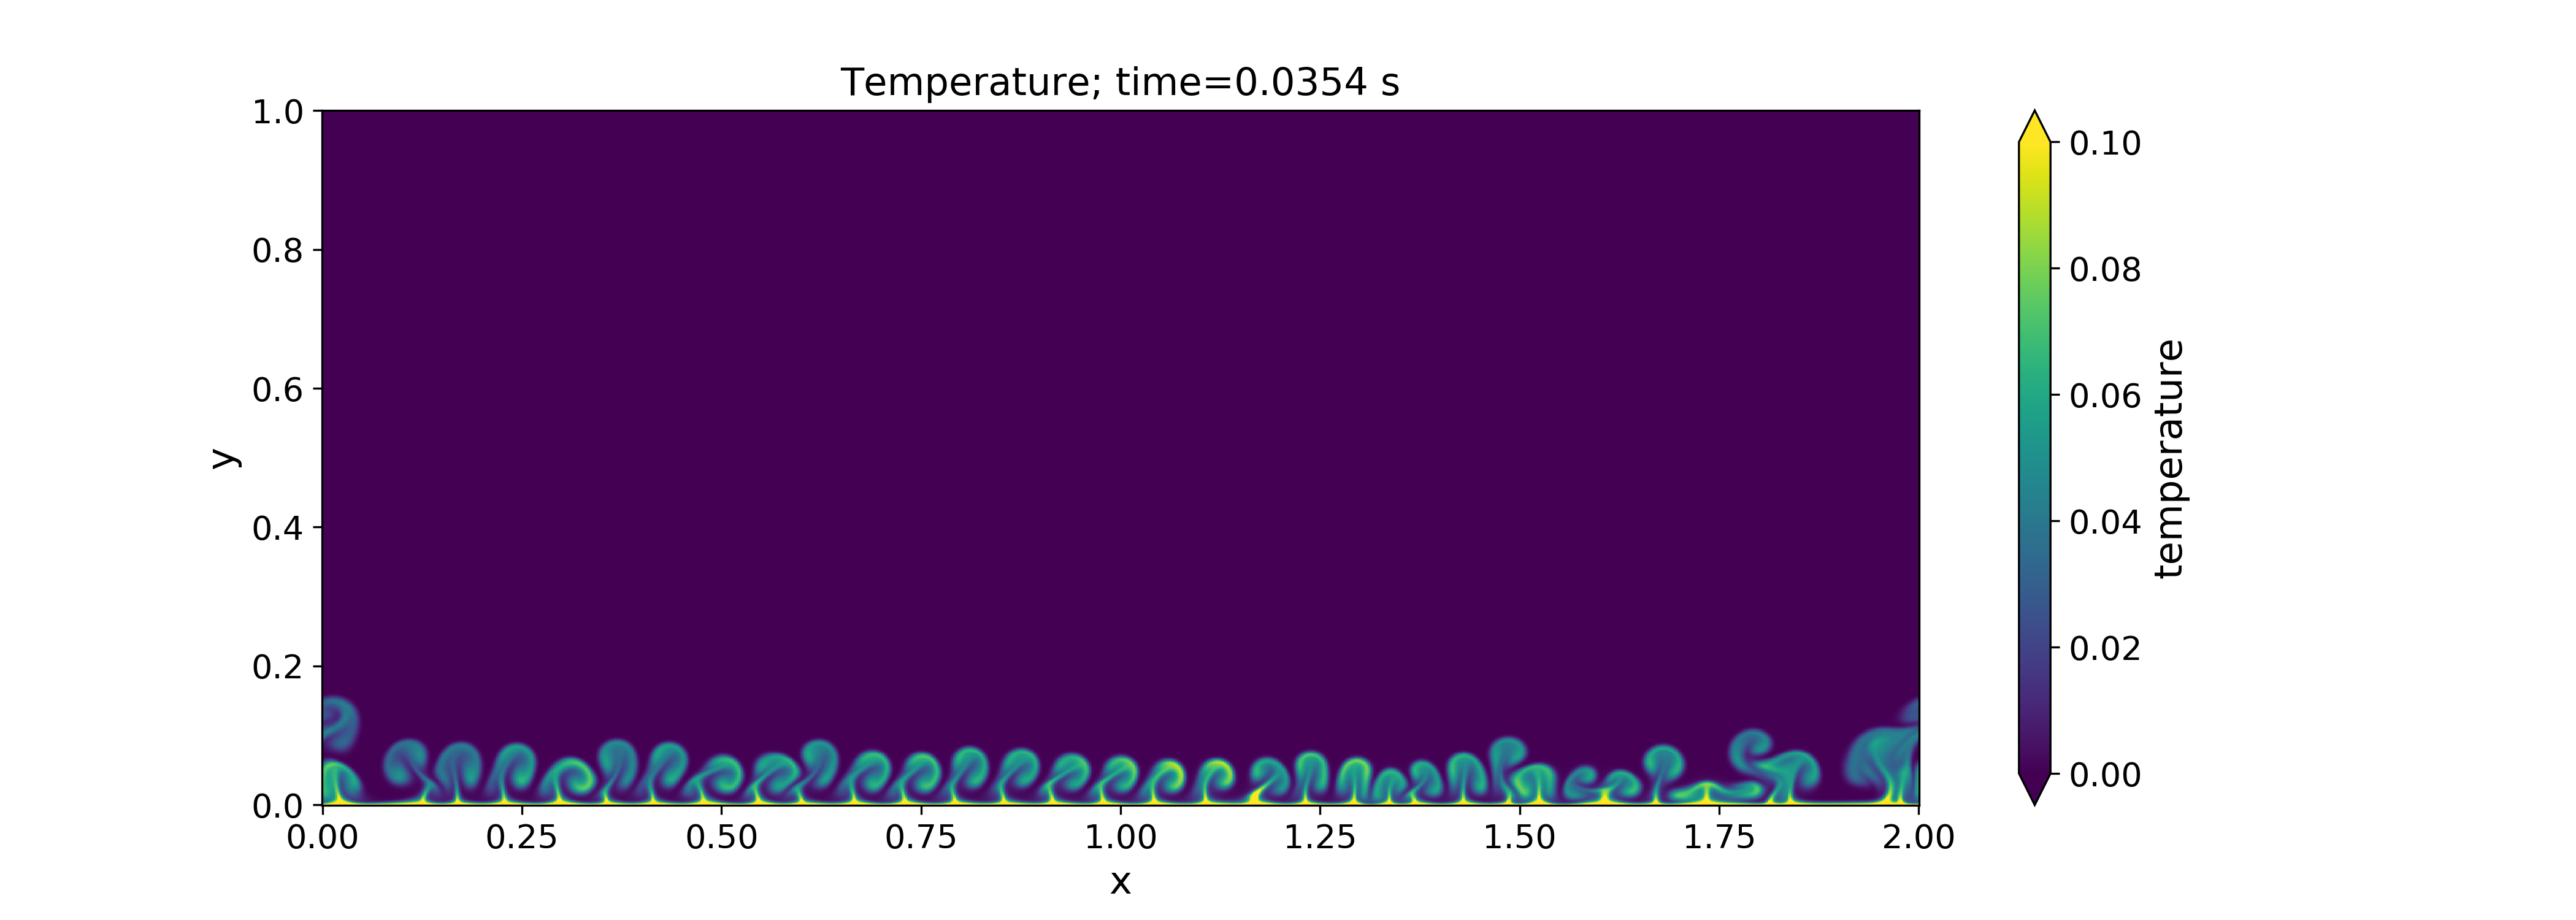
\includegraphics[scale=0.5]{temp_frame_037}
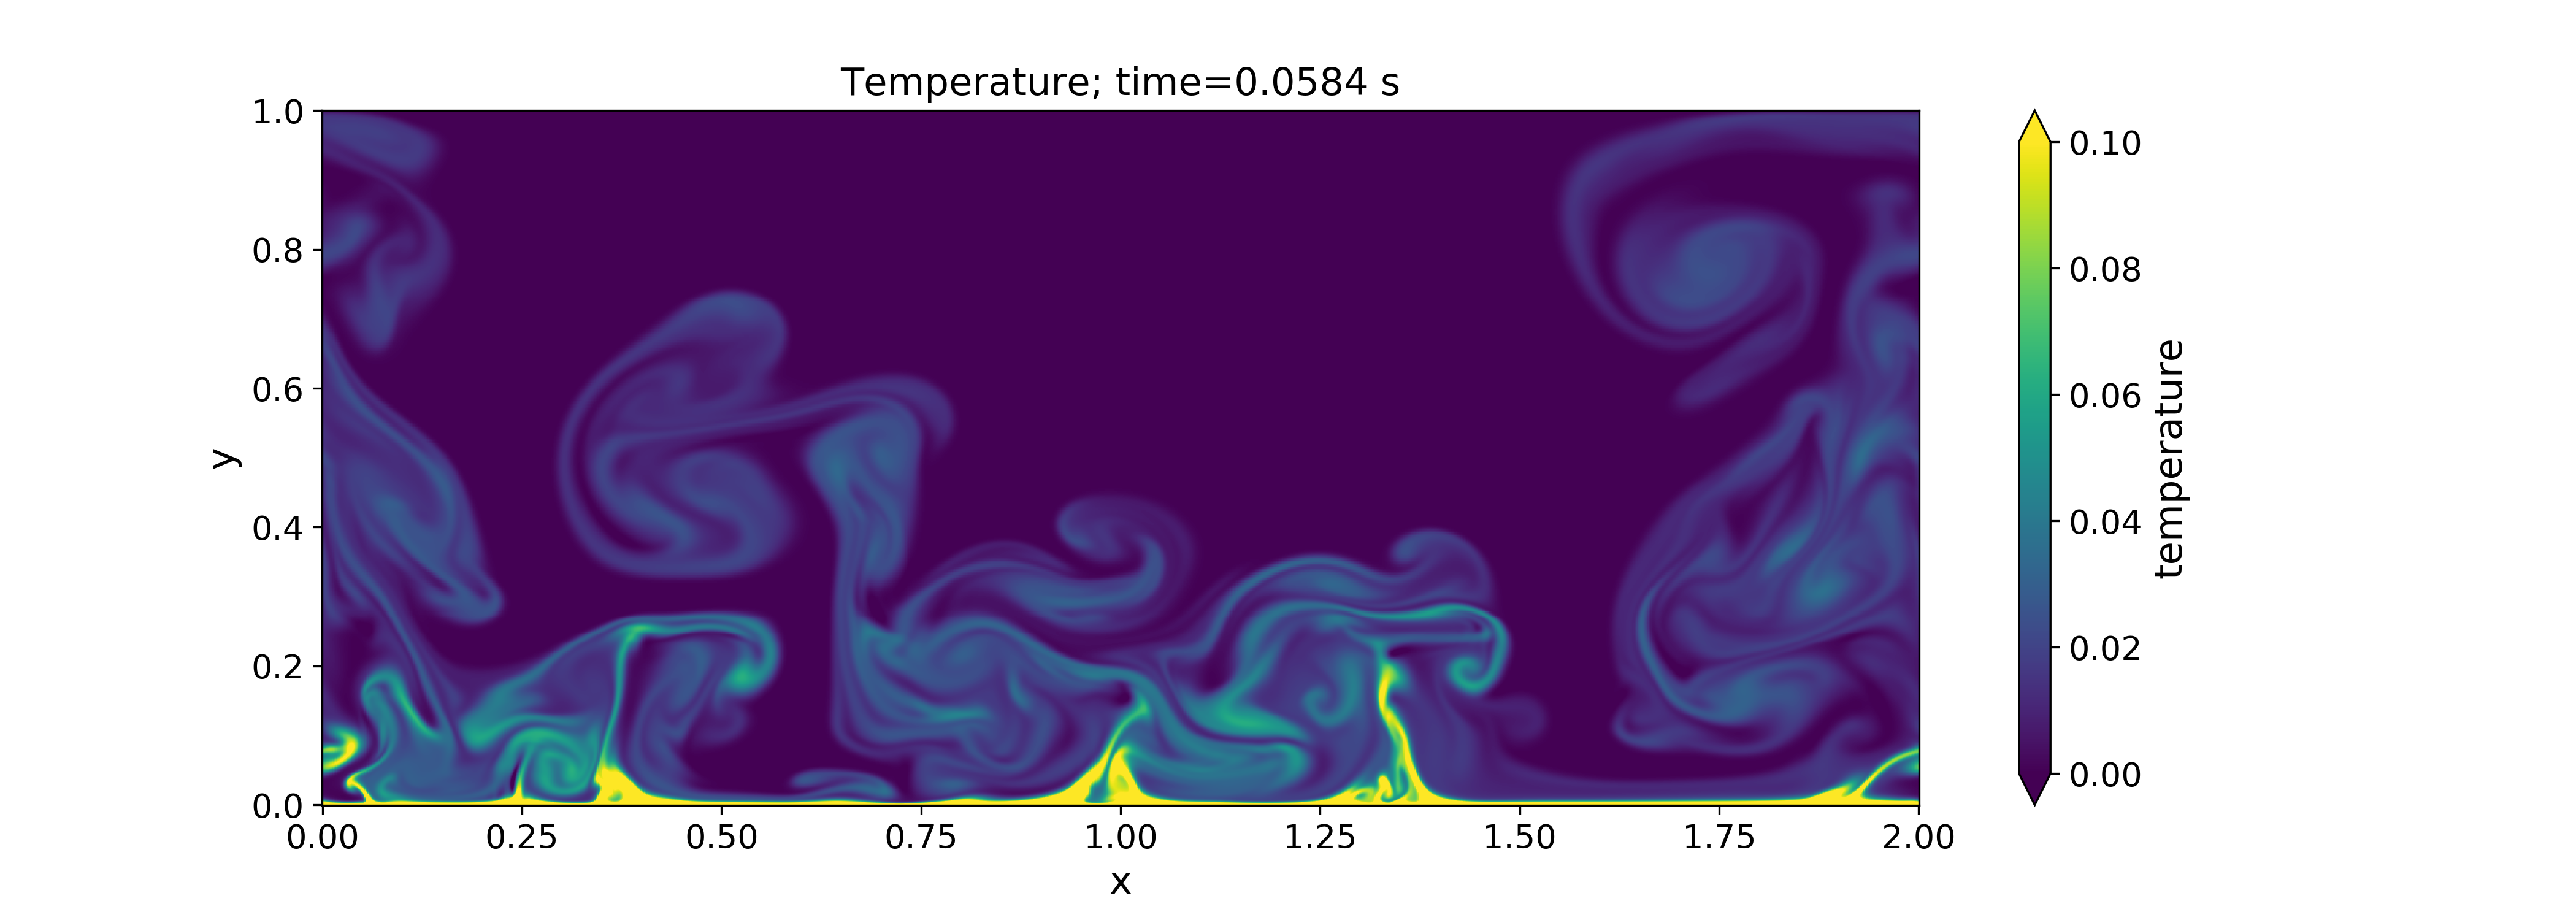
\includegraphics[scale=0.5]{temp_frame_060}
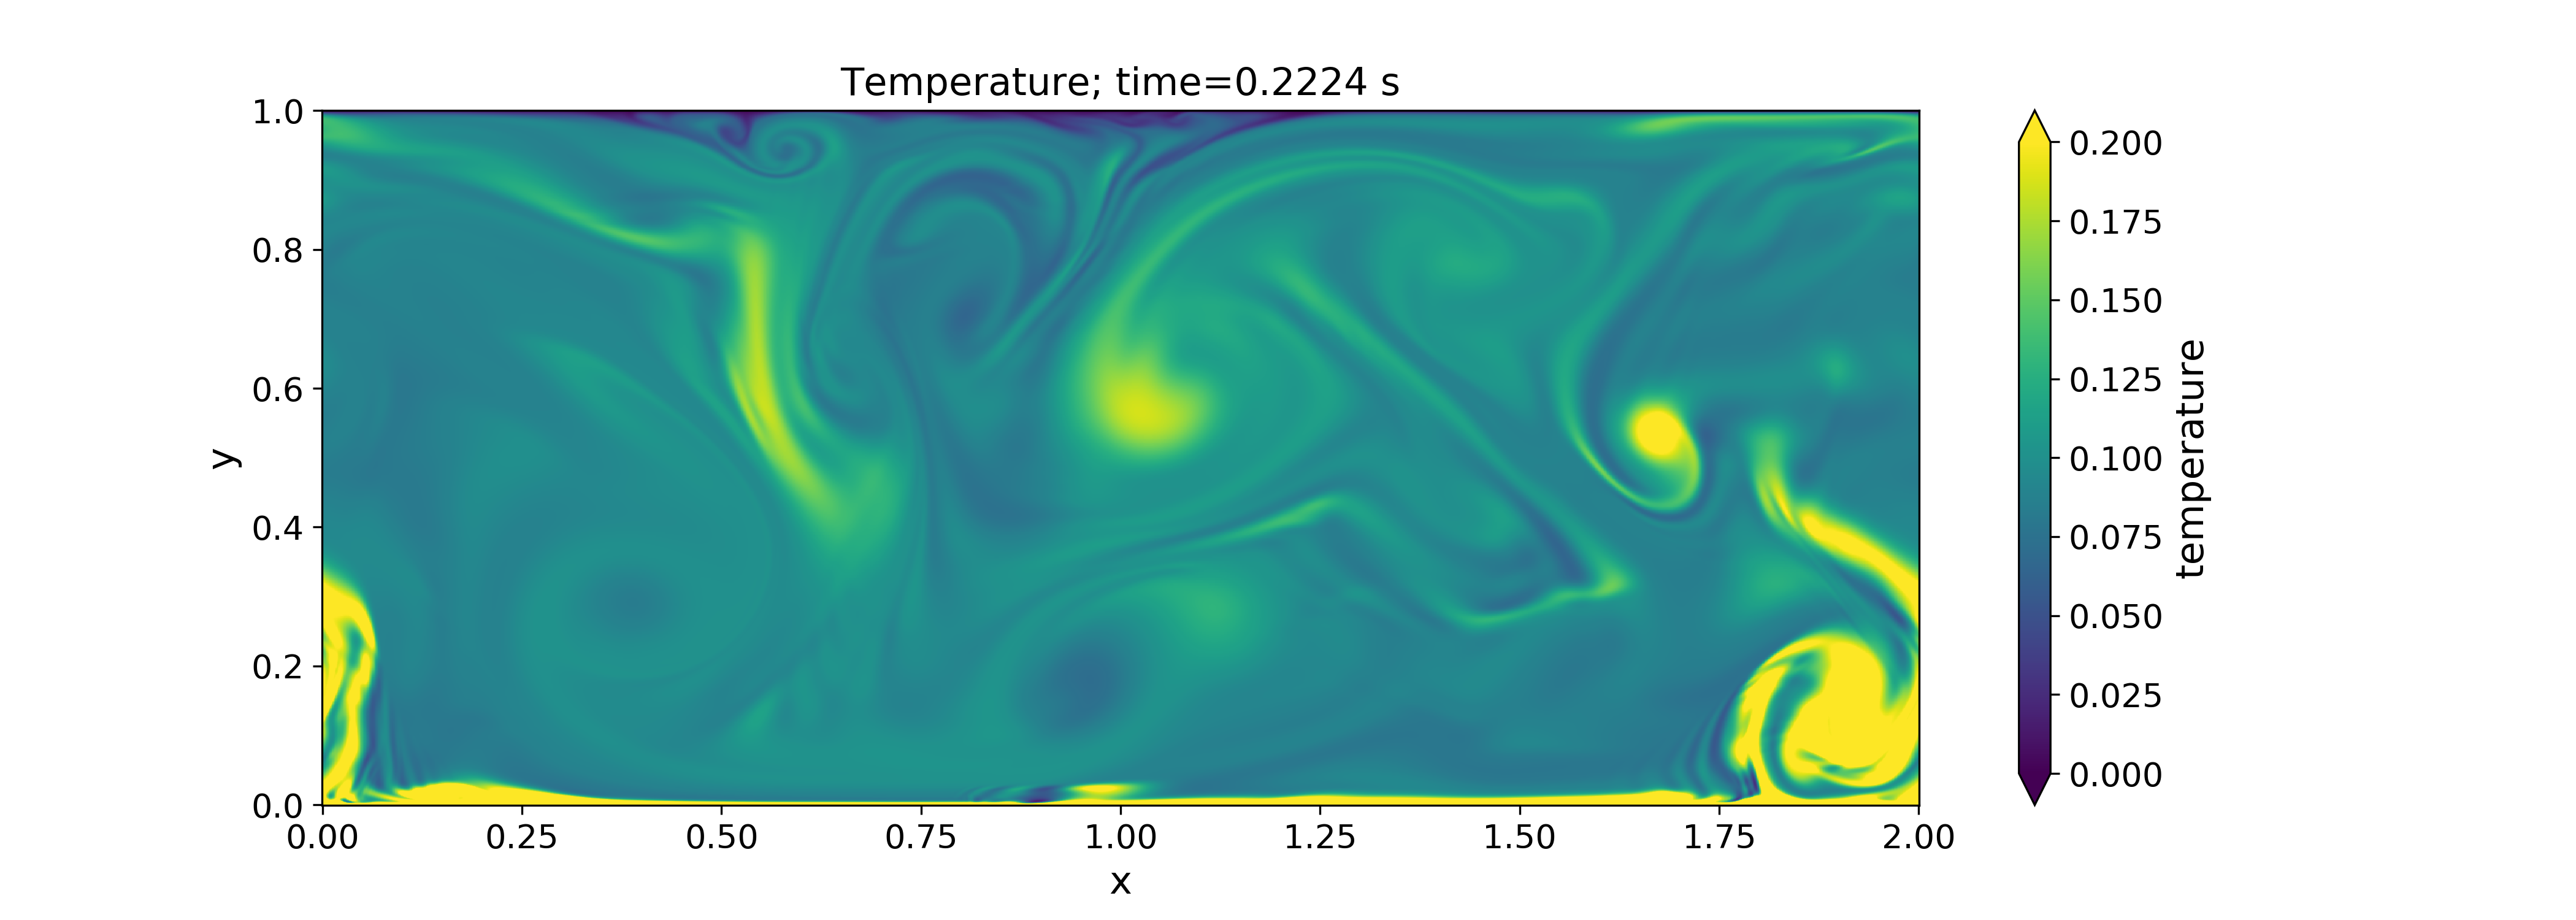
\includegraphics[scale=0.5]{temp_frame_224_vmax02}
\centering
\caption{Temperature field T(x, y) at different time. The last figure has a different colorbar scale, for better visualization.}
\end{figure}

Alternatively, the same temperature field can be plotted with filled-contours. The darkest region are small negative values (around $-10^{-10}$), because we do not cap negative values in the input XML file. Otherwise, the overall pattern is consistent with the previous plot.

\begin{figure}[H]
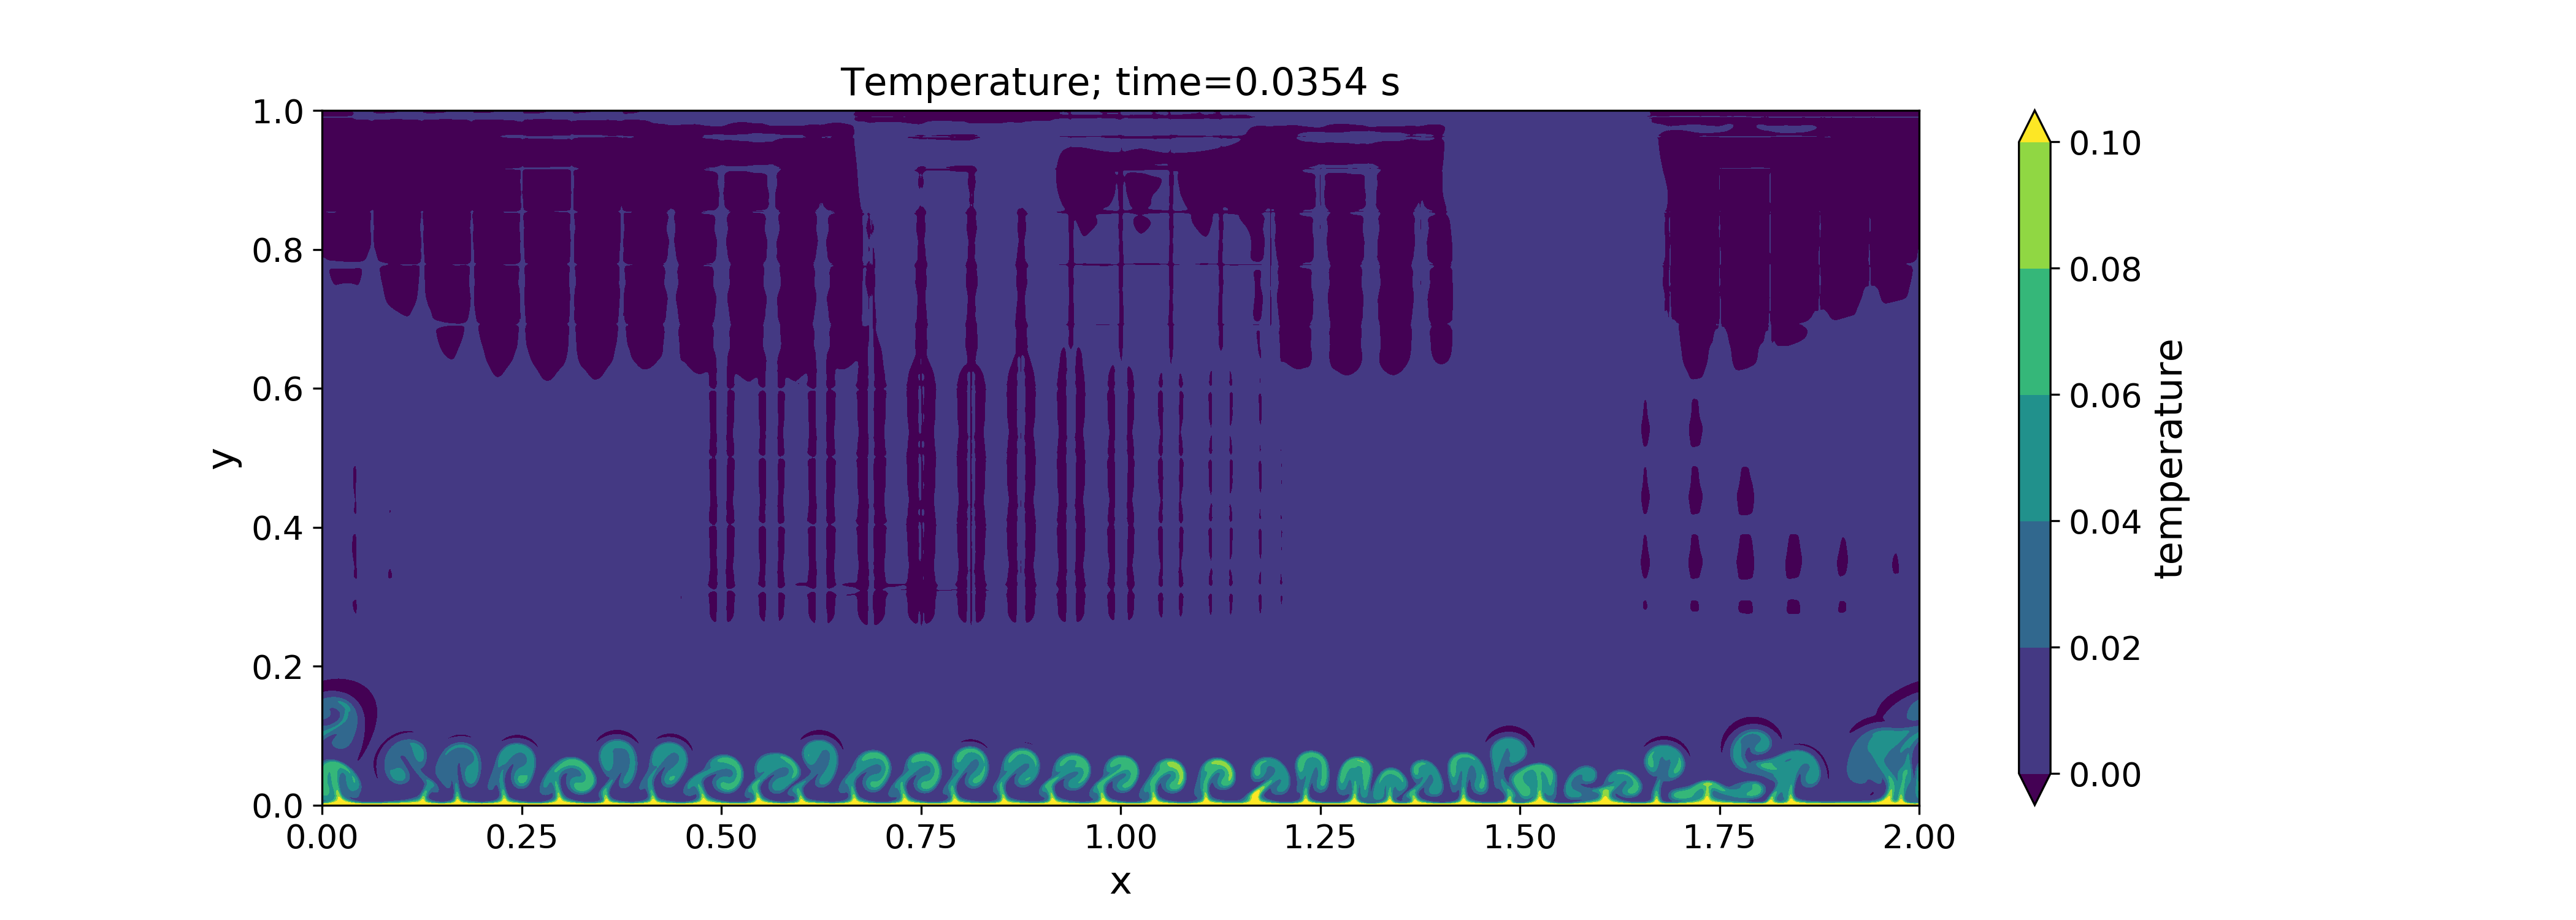
\includegraphics[scale=0.5]{contour_frame_037}
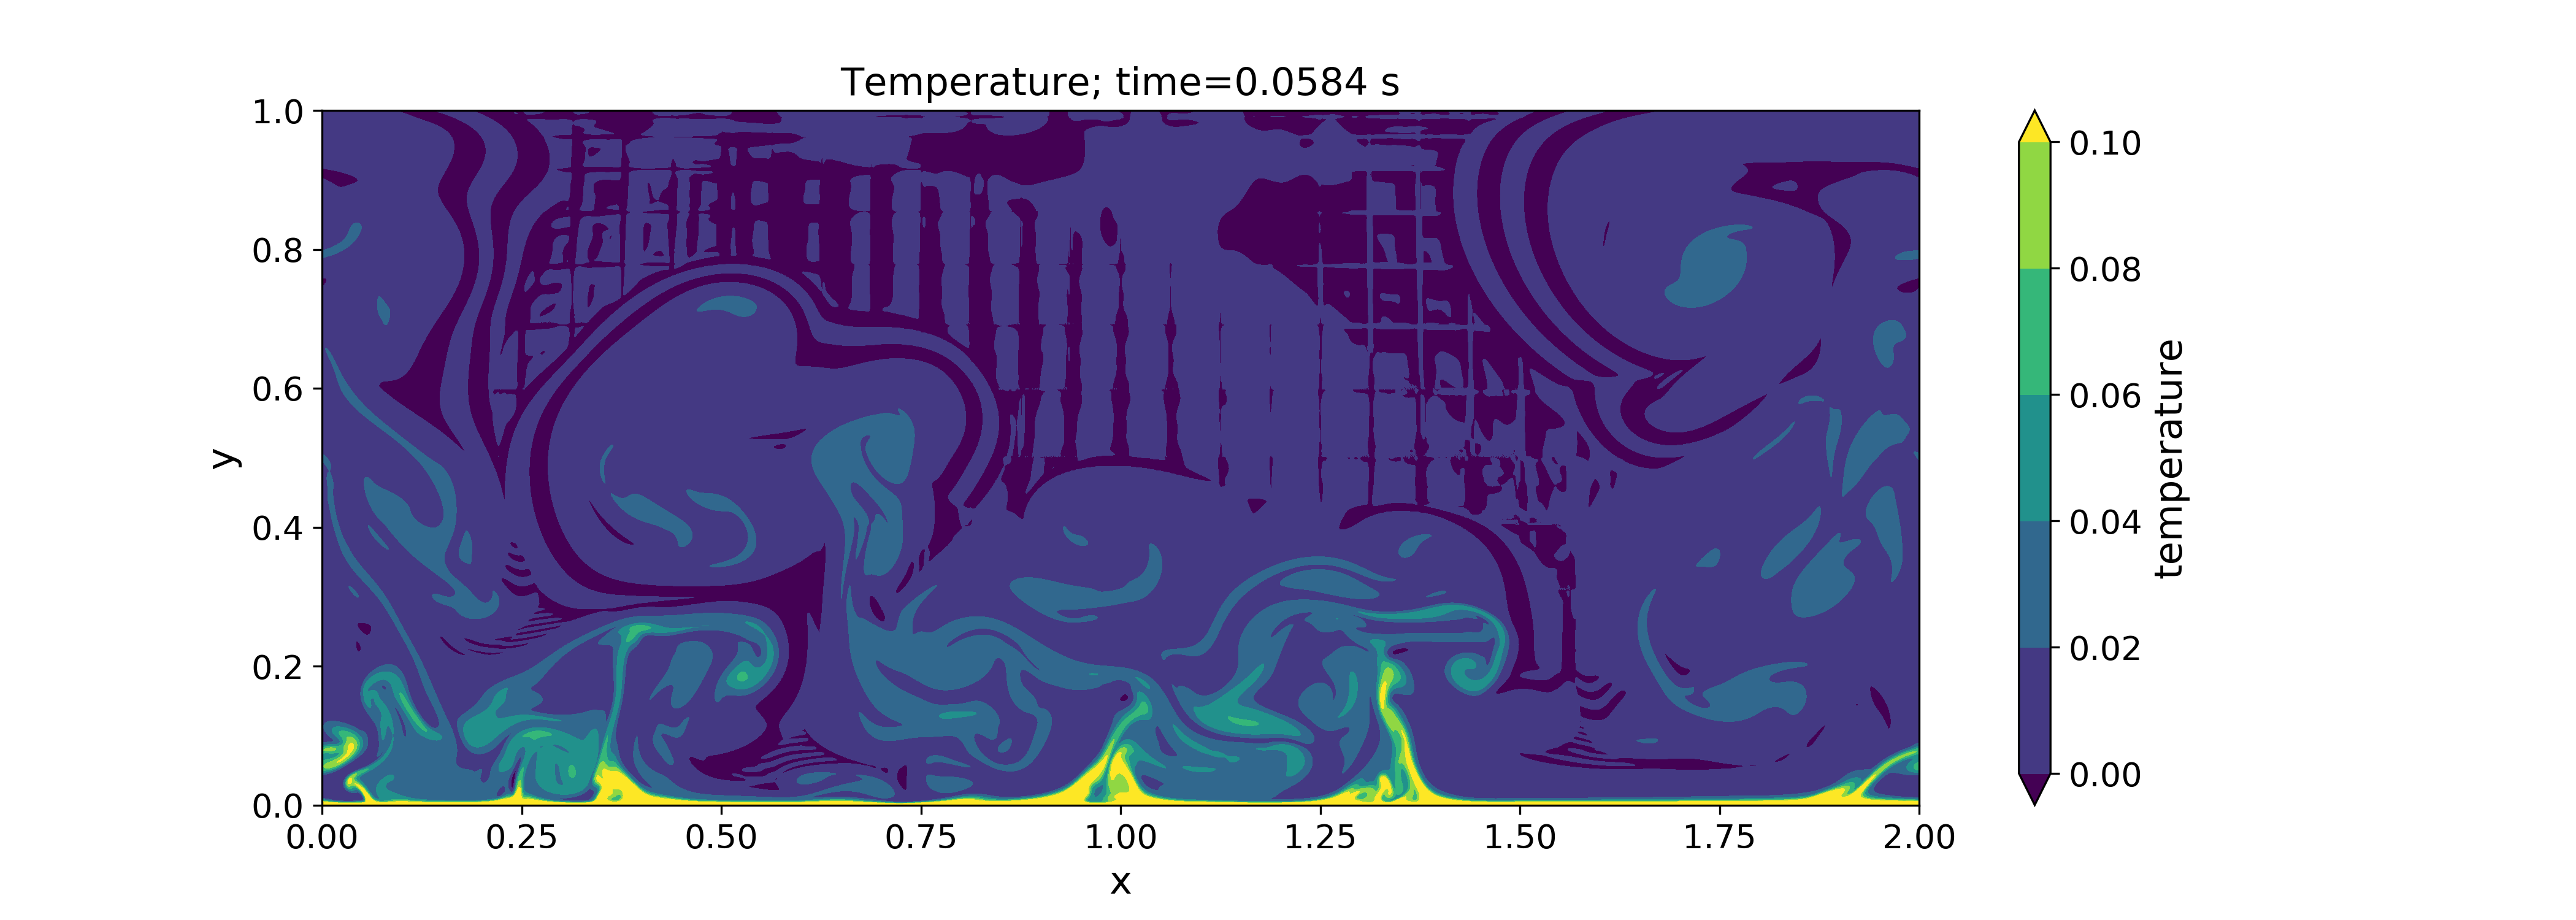
\includegraphics[scale=0.5]{contour_frame_060}
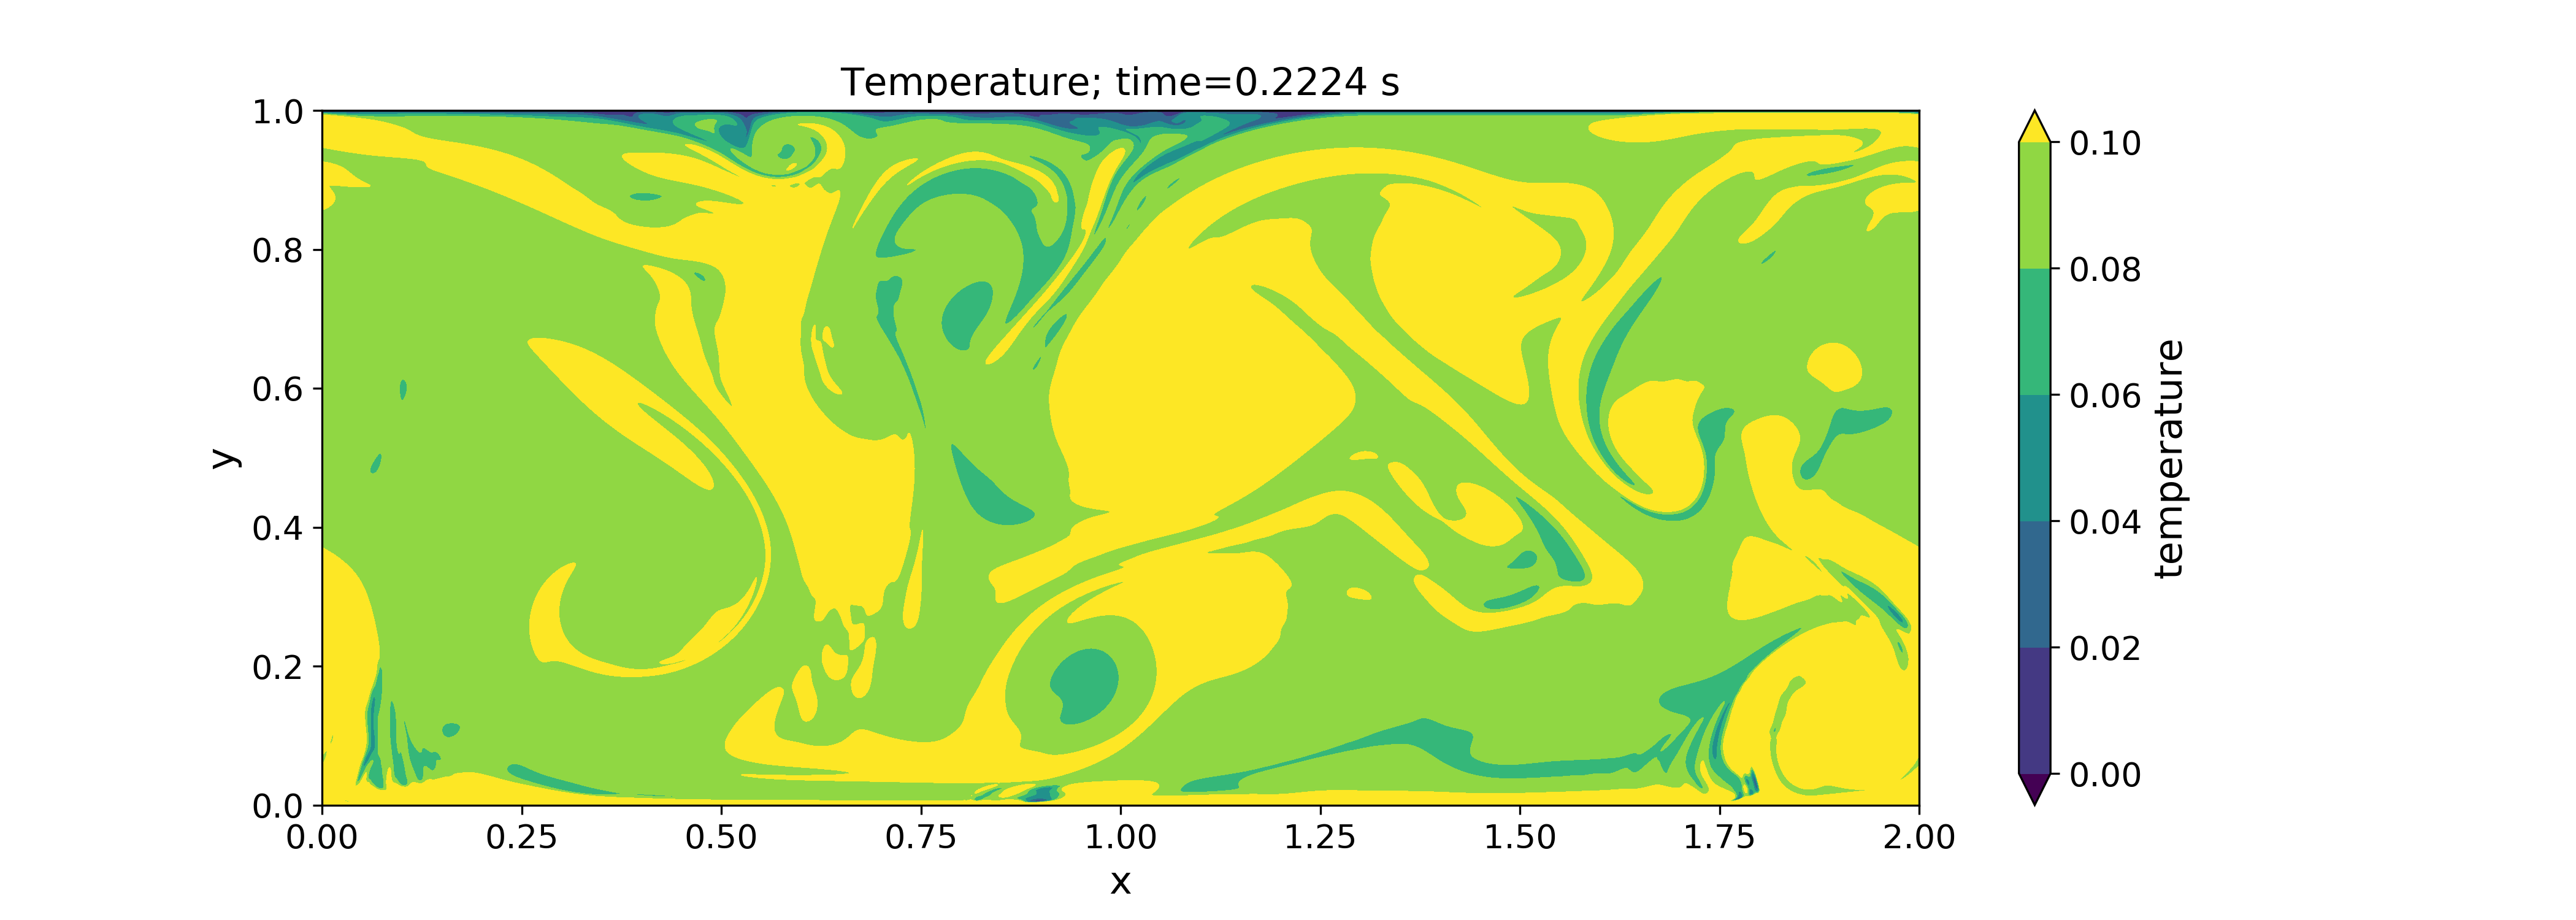
\includegraphics[scale=0.5]{contour_frame_224}
\centering
\caption{Filled-contour plot of temperature field T(x, y) at different time. Darkest regions indicate slight negative values.}
\end{figure}

\subsubsection{Temperature profile}

Then we turn to the vertical profile of temperature. Below shows the temperature profile averaged over x and t.

\begin{figure}[H]
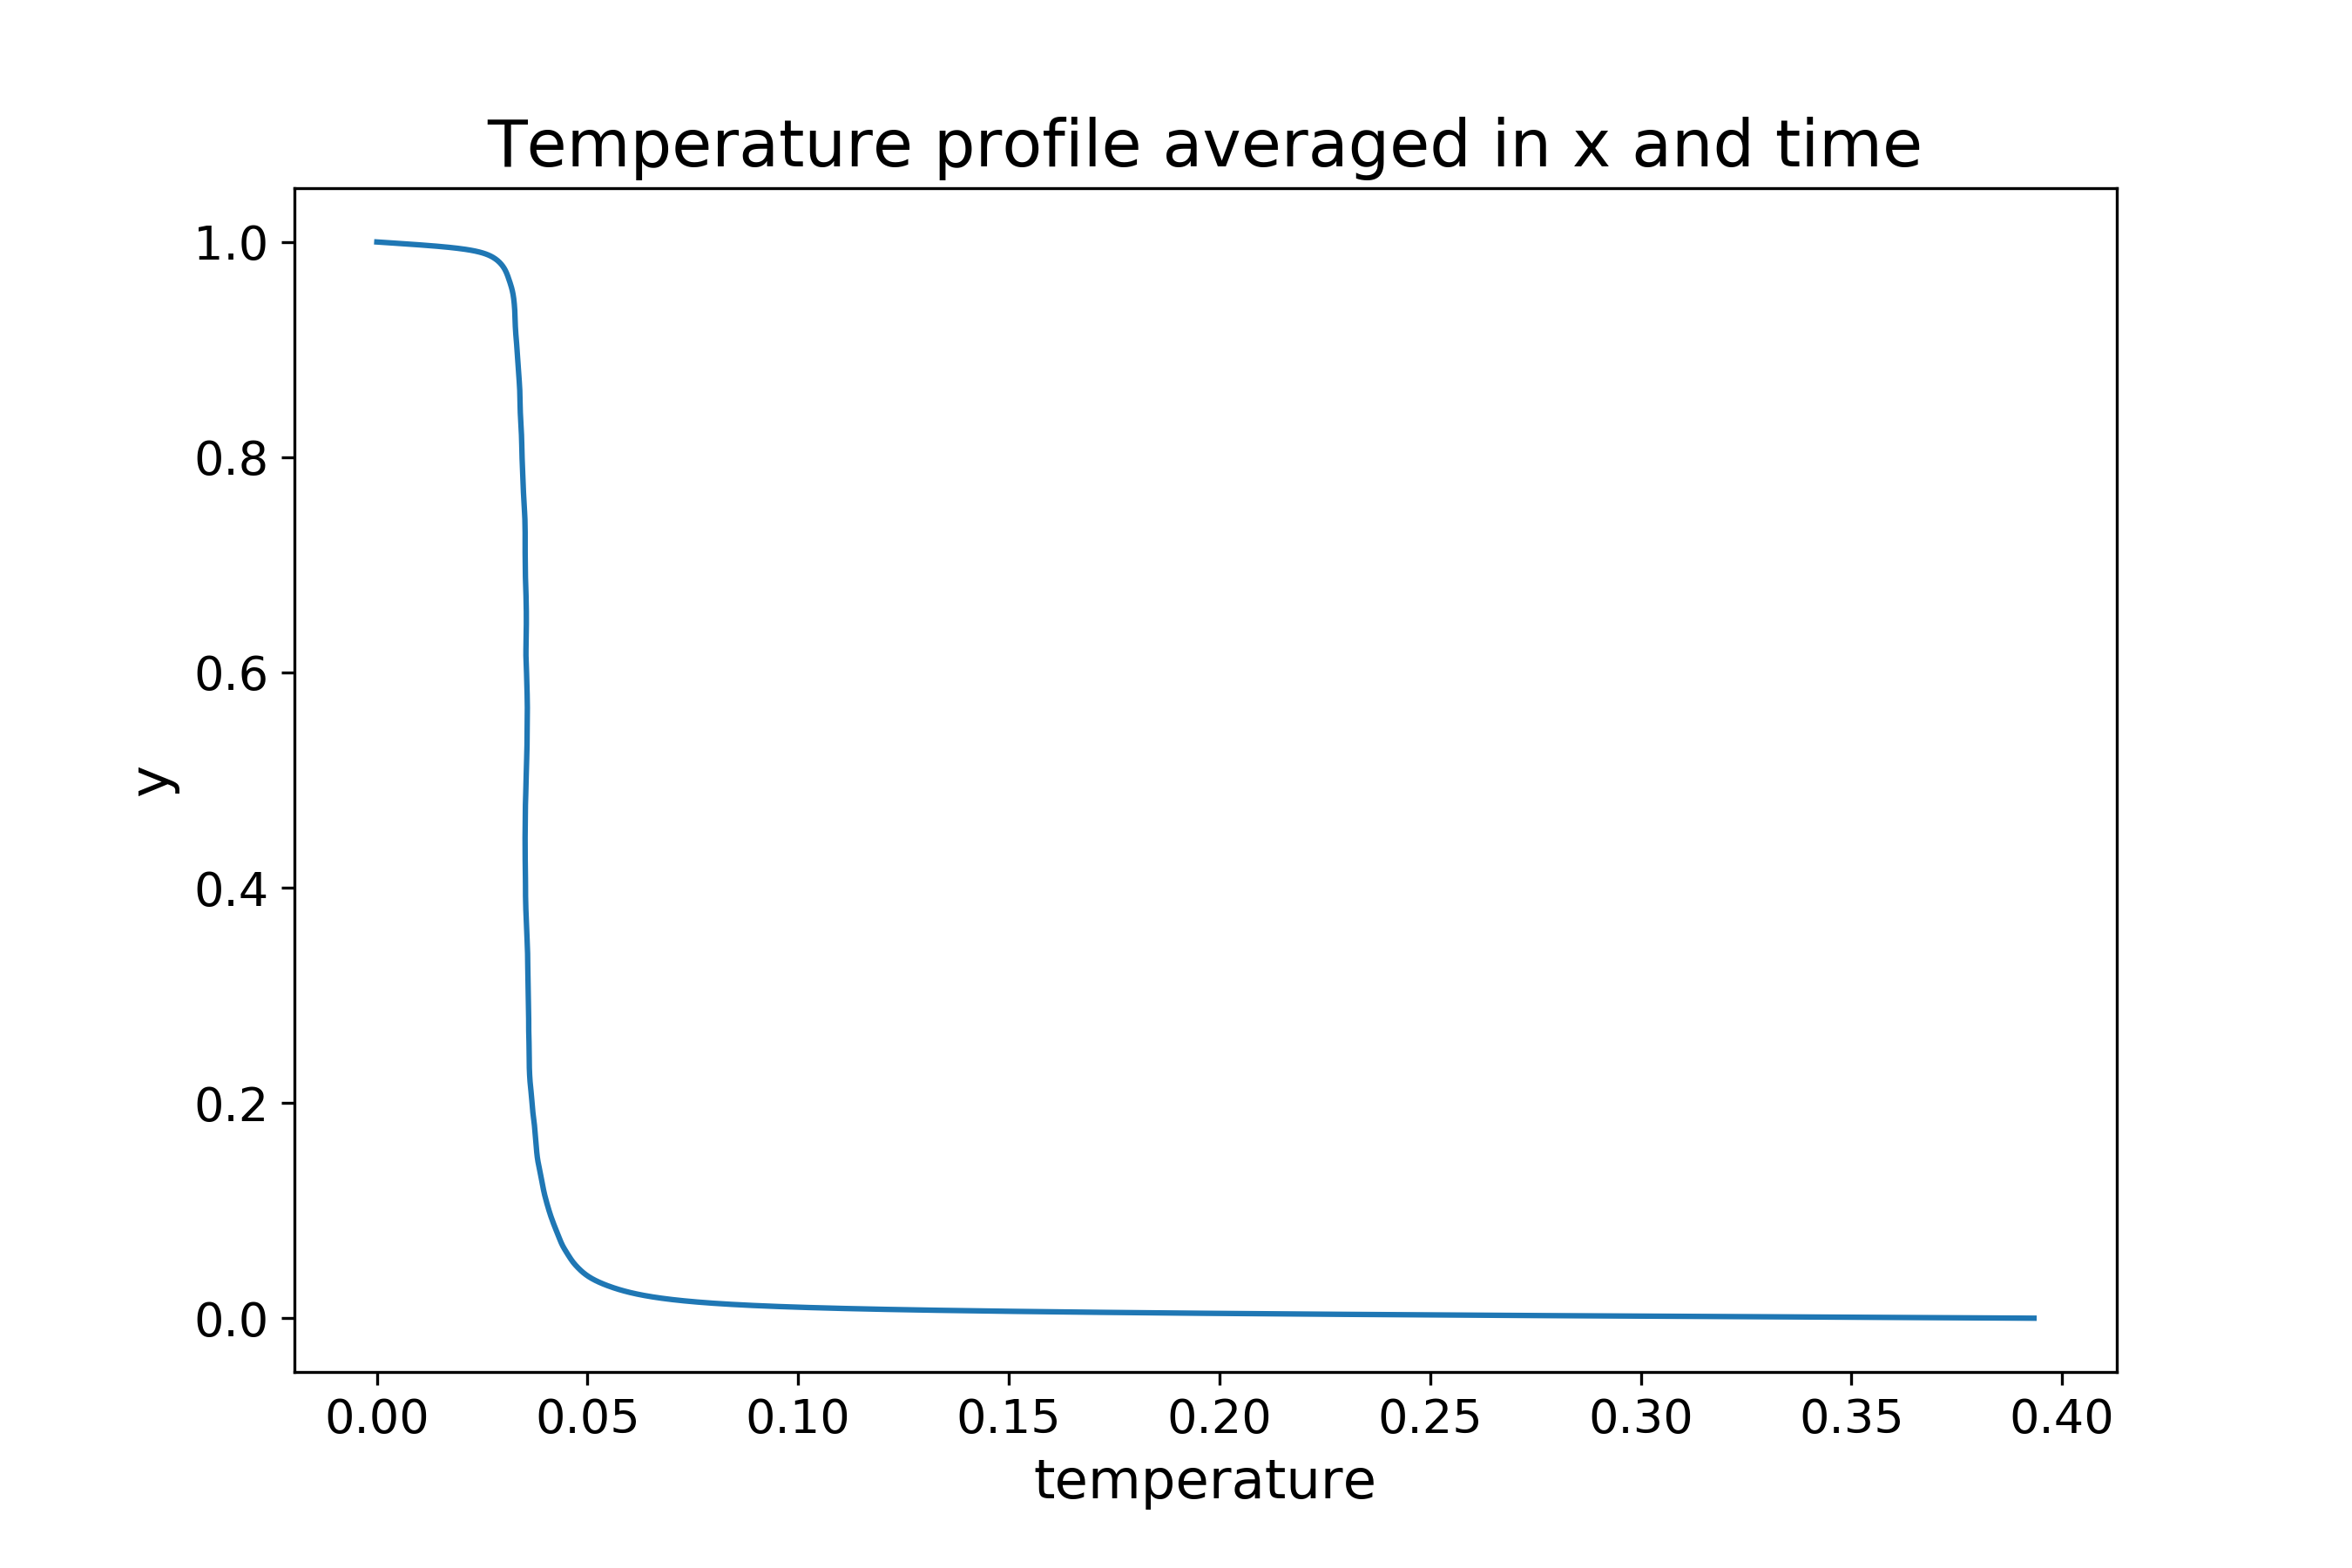
\includegraphics[scale=0.5]{temperature_y}
\centering
\caption{Temperature profile T(y) (averaged over x and t)}
\end{figure}

The average profile shows the temperature gradient but not the dynamics of the system. To show the time evolution, we plot the instant temperature profile at different time slots, as available in the video in the slides. Here only plots the last time frame. It shows a step-function-like front that keeps moving to the right (i.e. temperature increases). If the simulation continues, the "front" of the profile will finally reach $T=0.5$, which is the average of bottom and top temperature.

\begin{figure}[H]
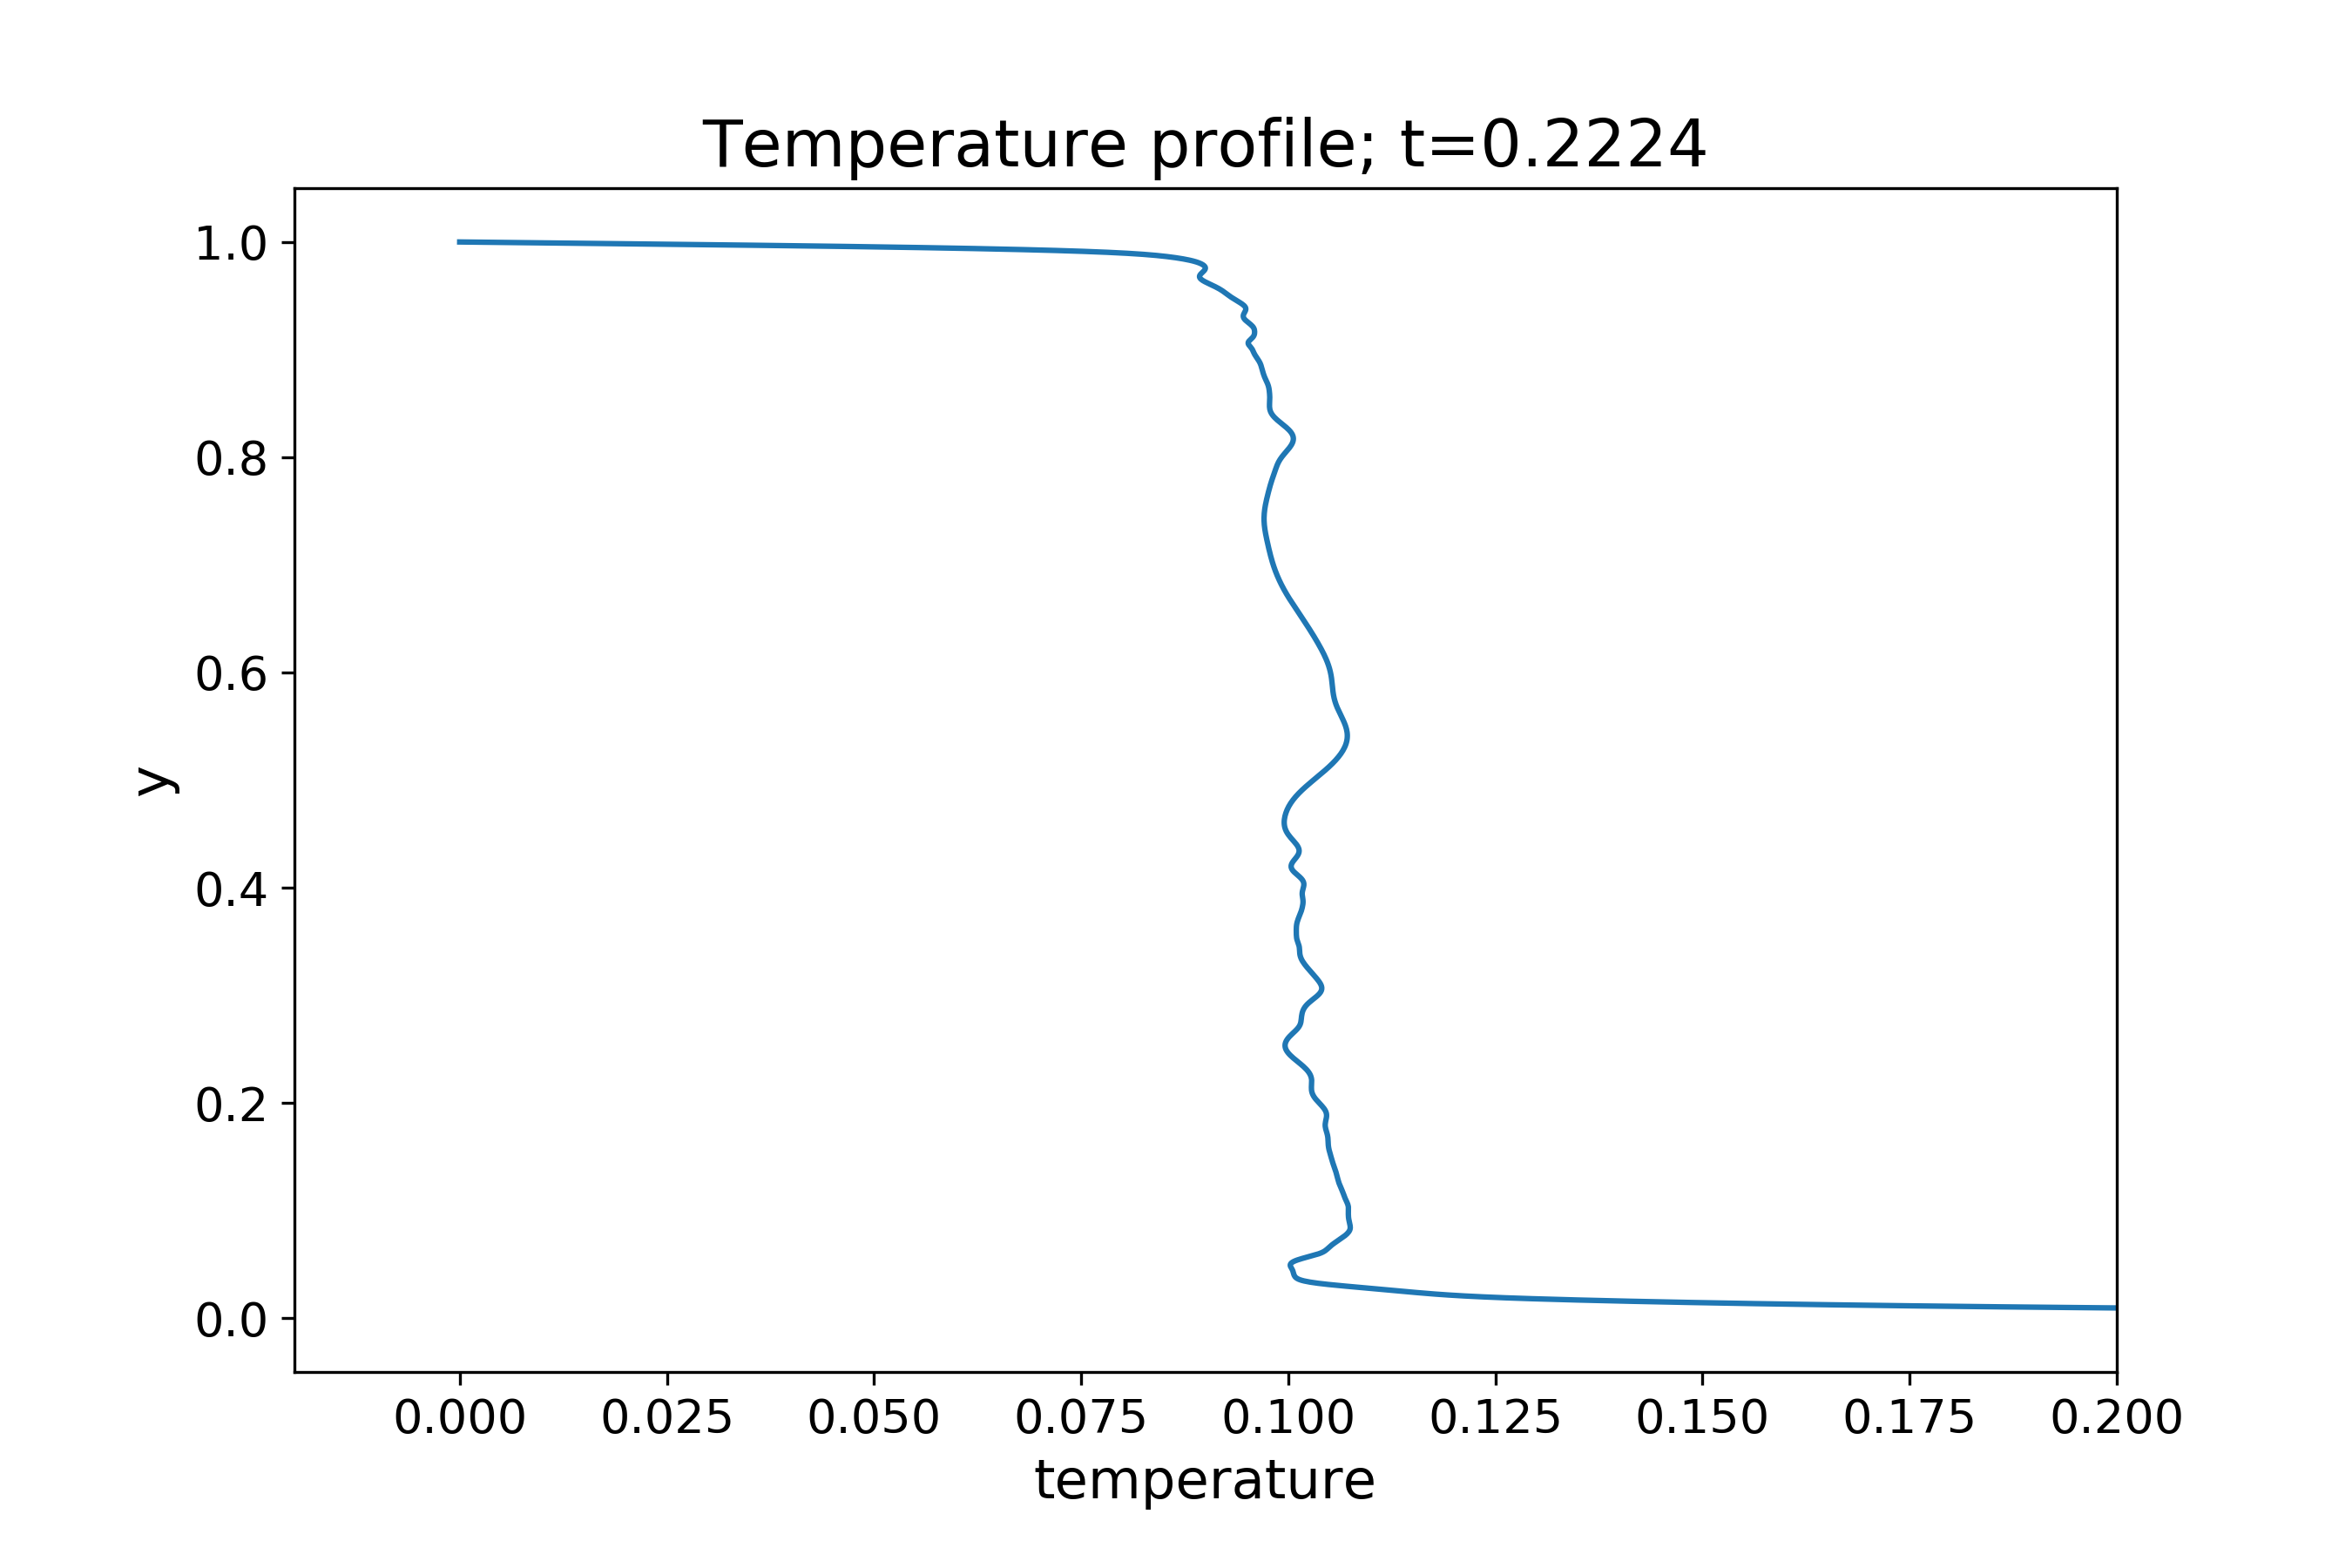
\includegraphics[scale=0.5]{profile_frame_224}
\centering
\caption{Temperature profile T(y) (averaged over x) at a single time frame. The "front" keeps moving to the right.}
\end{figure}

We can also put the profiles (averaged over x) together into one figure, with the x-axis indicating time evolution. 

\begin{figure}[H]
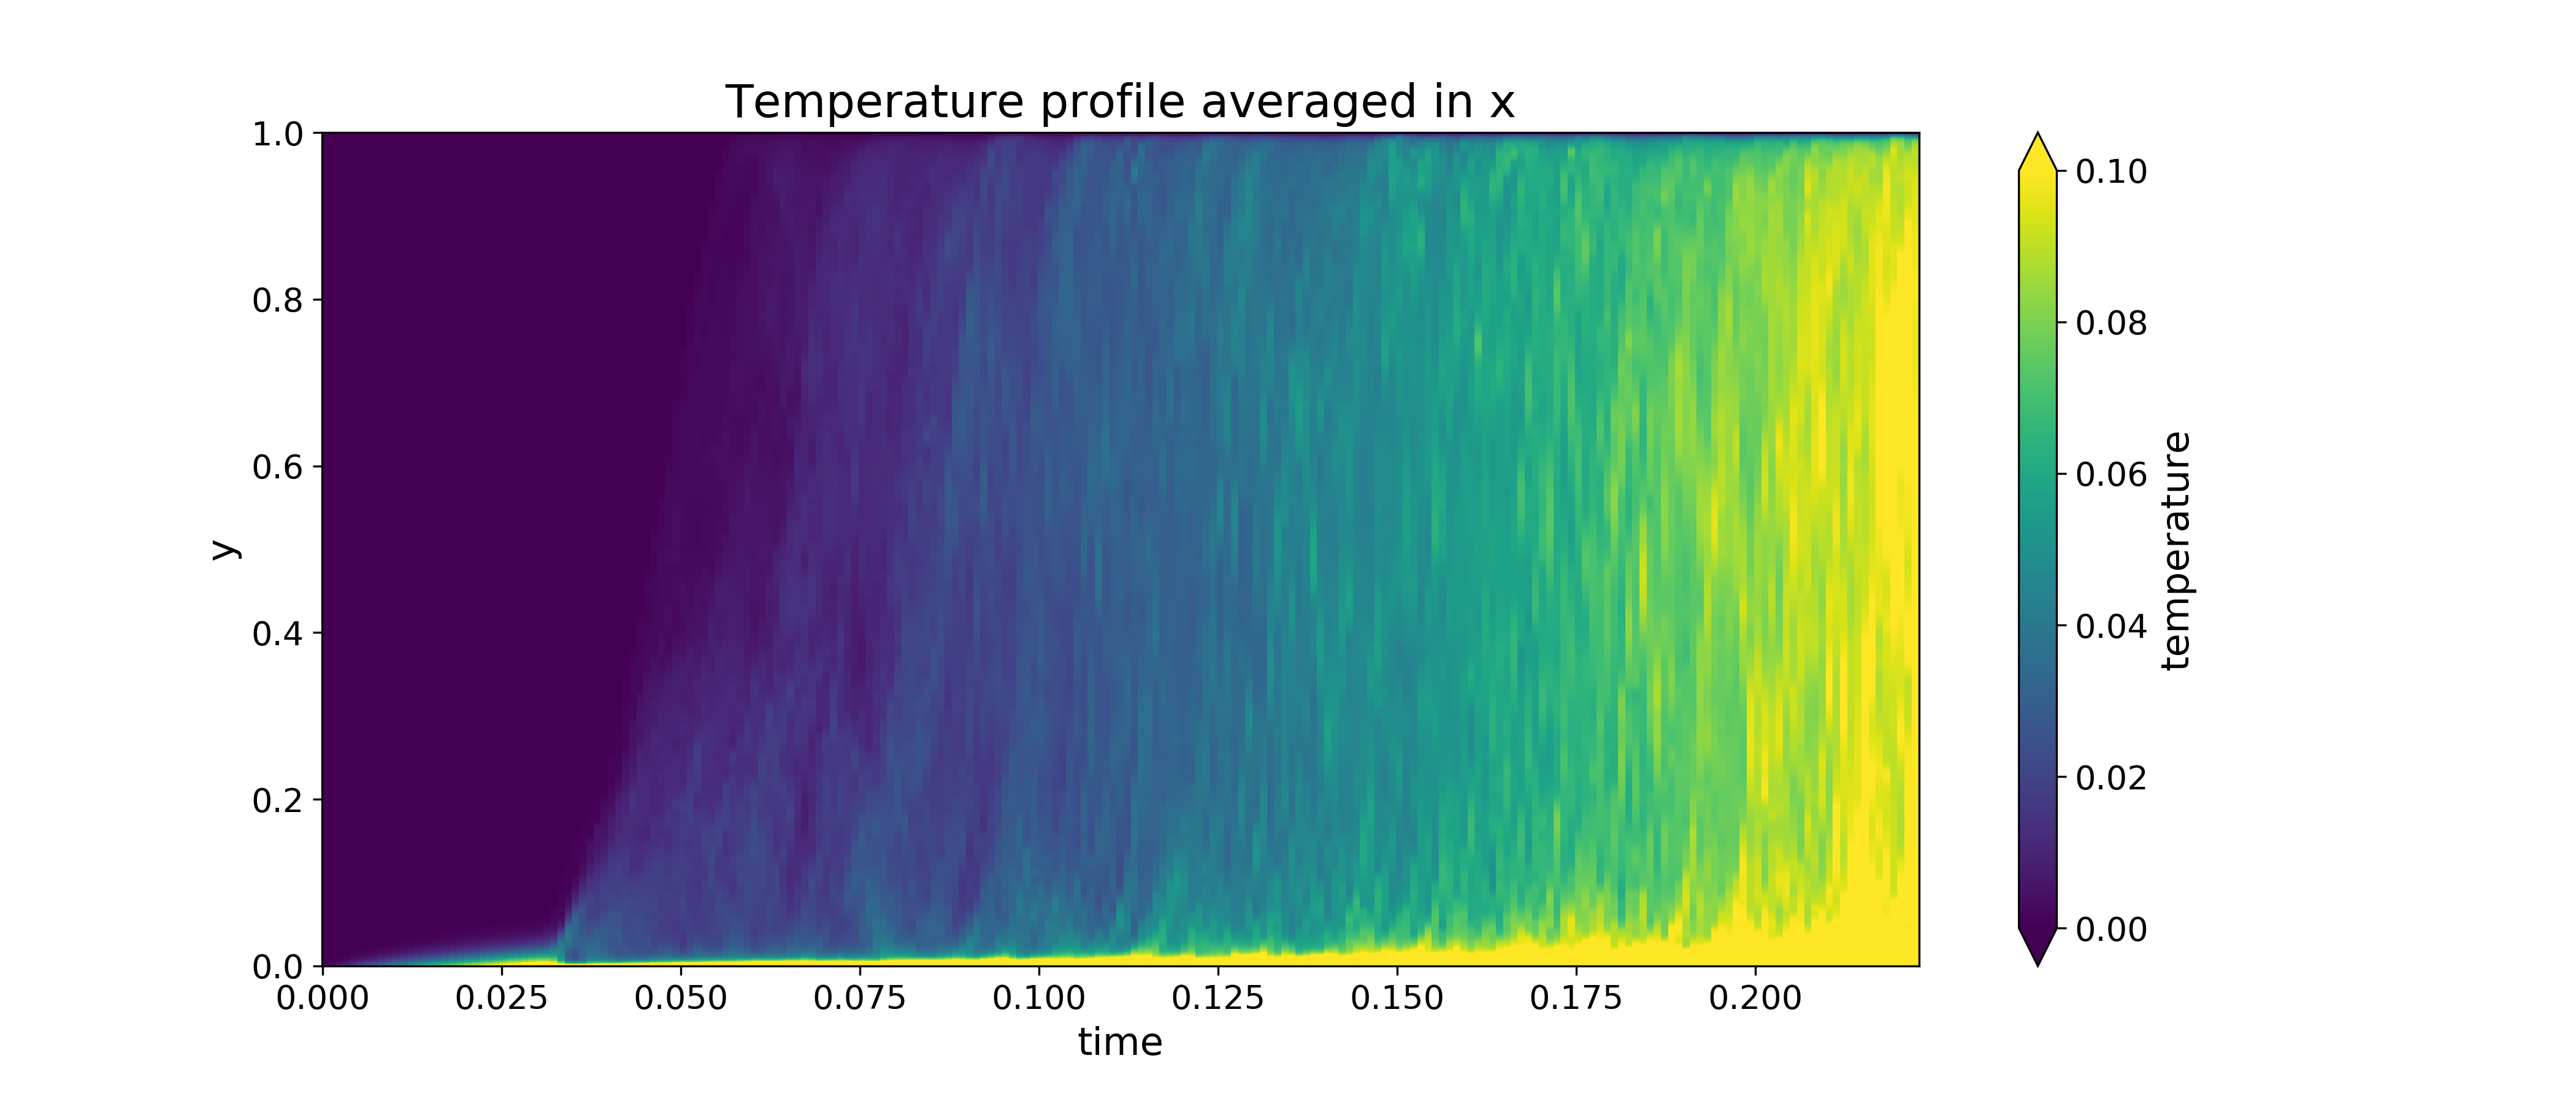
\includegraphics[scale=0.5]{temperature_y_time}
\centering
\caption{Temperature profile T(y, t) (averaged over x, change with time)}
\end{figure}

\subsubsection{Boundary condition}

The boundary condition $T(y=0)$ starts with 0 and gradually reaches 1. This is consistent with the input XML file. Given our relatively short simulation period, the bottom temperature at the last time step is still far from the steady state $T=1$.

\begin{figure}[H]
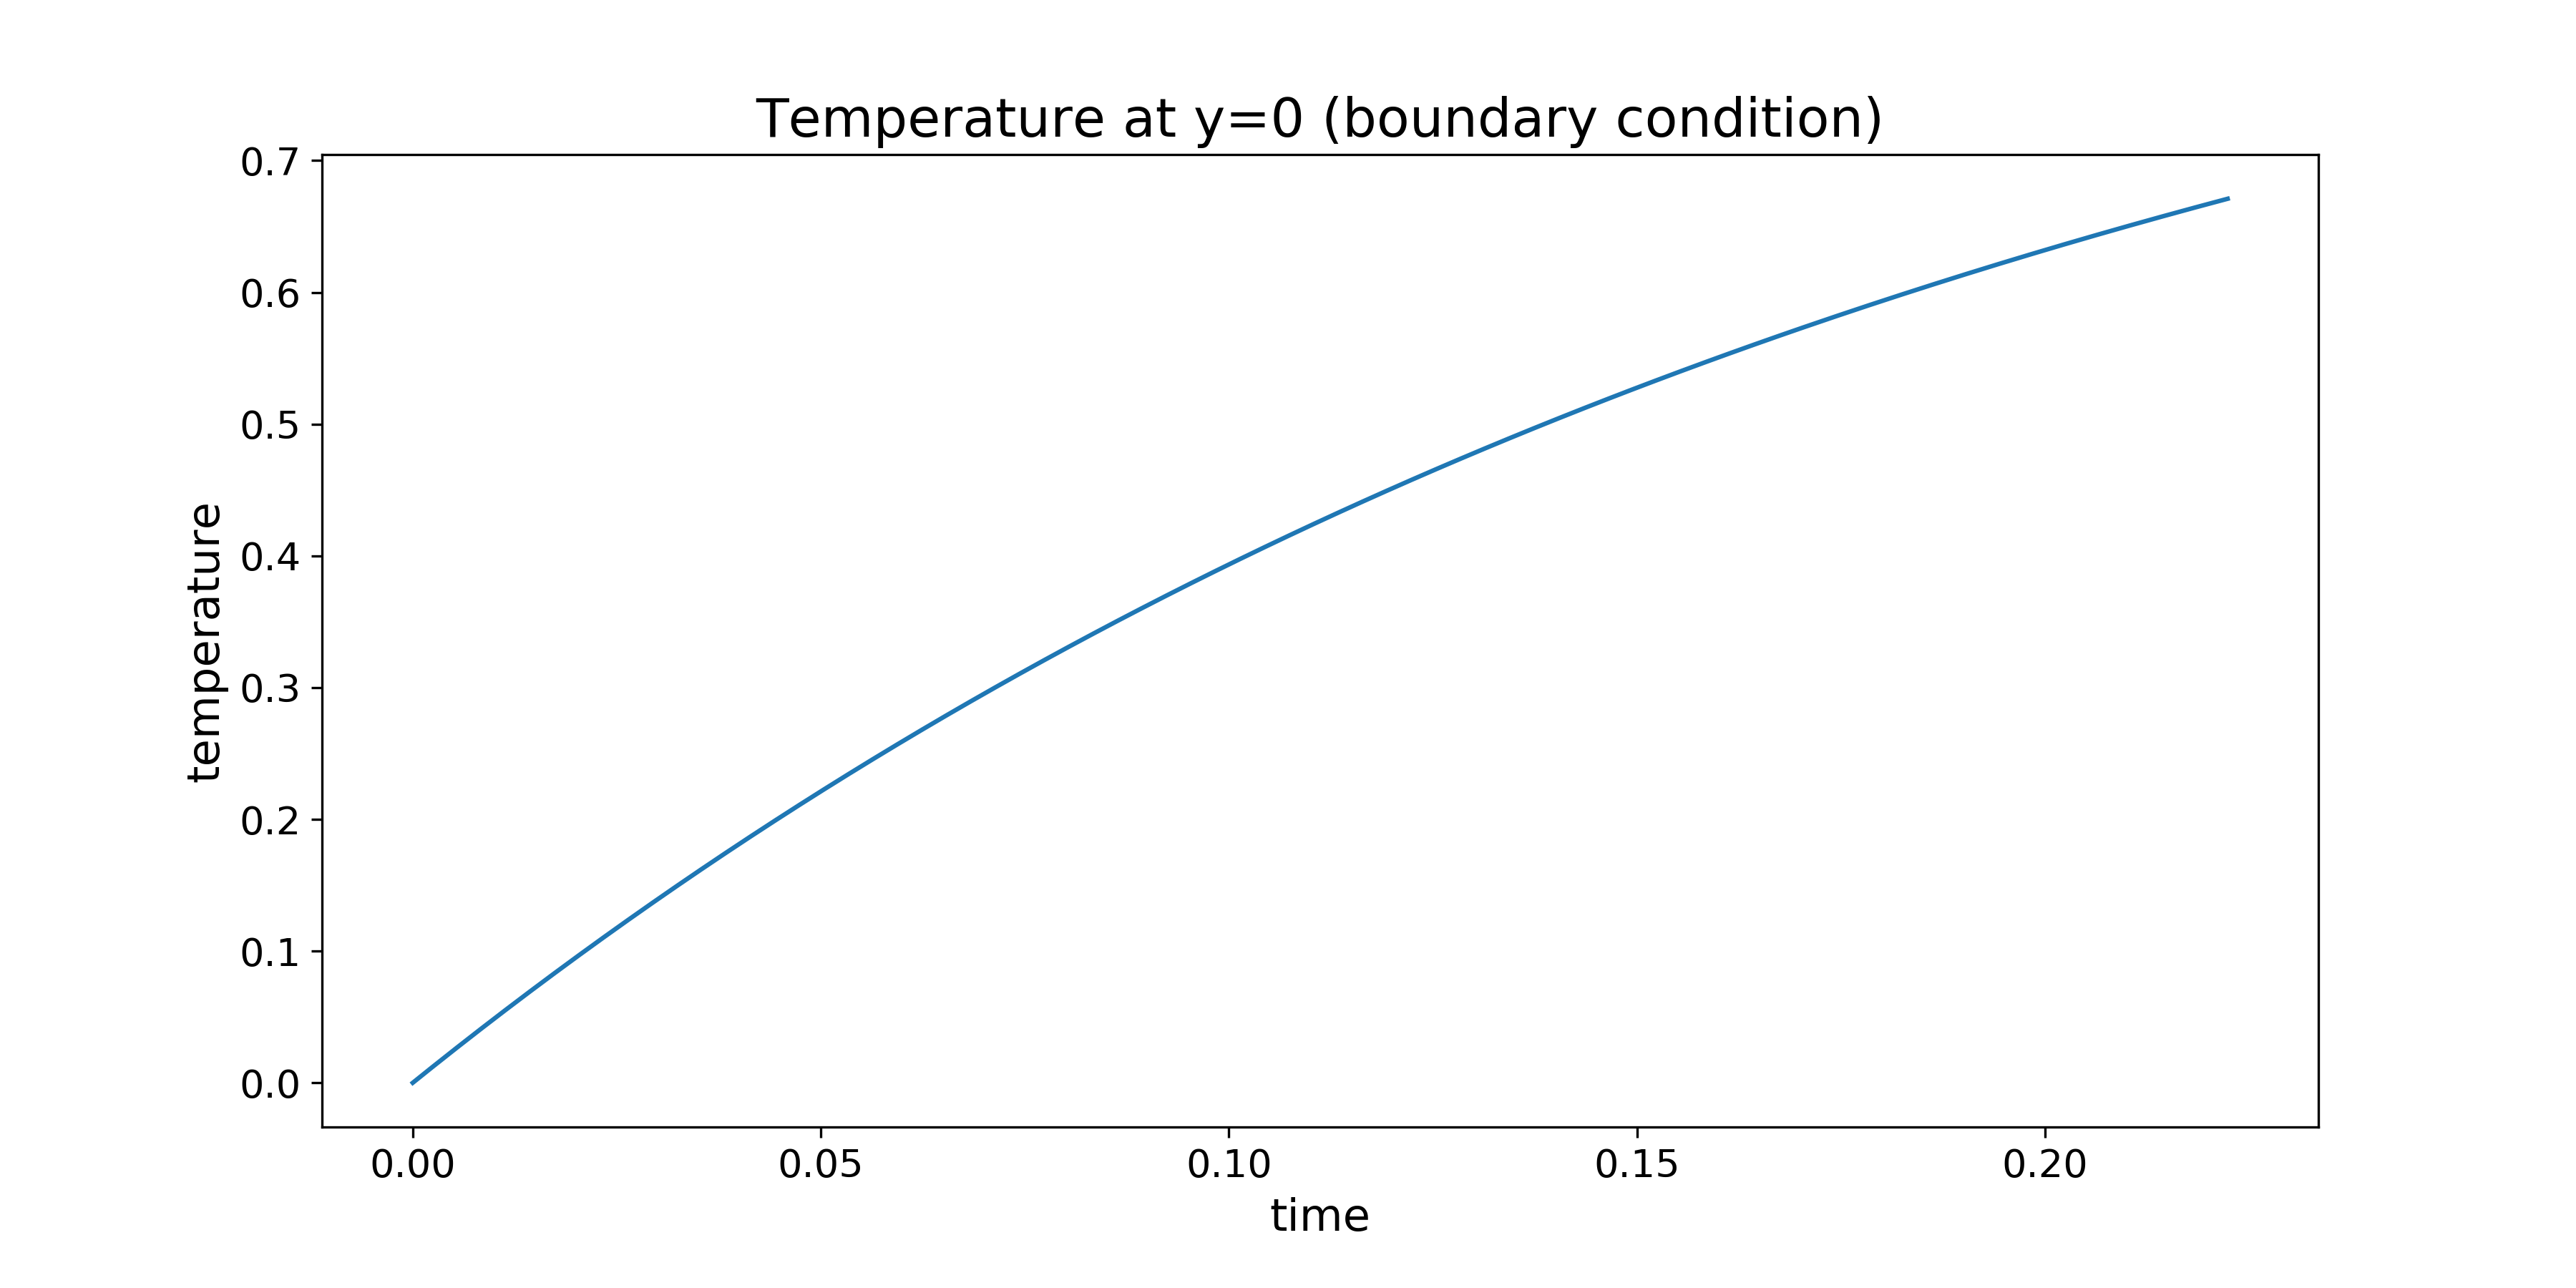
\includegraphics[scale=0.5]{y_bottom}
\centering
\caption{Boundary condition T(y=0)}
\end{figure}

\subsection{Schlieren visualization}

We then compute the Schlieren field from the temperature, using the formula:

\begin{align}
Sch = exp(-k\frac{|\nabla T|}{max(|\nabla T|)})
\end{align}

To get rich visualizations, we use a relatively large $k=50$. With small $k$, most areas will be dark (values close to 1).

\begin{figure}[H]
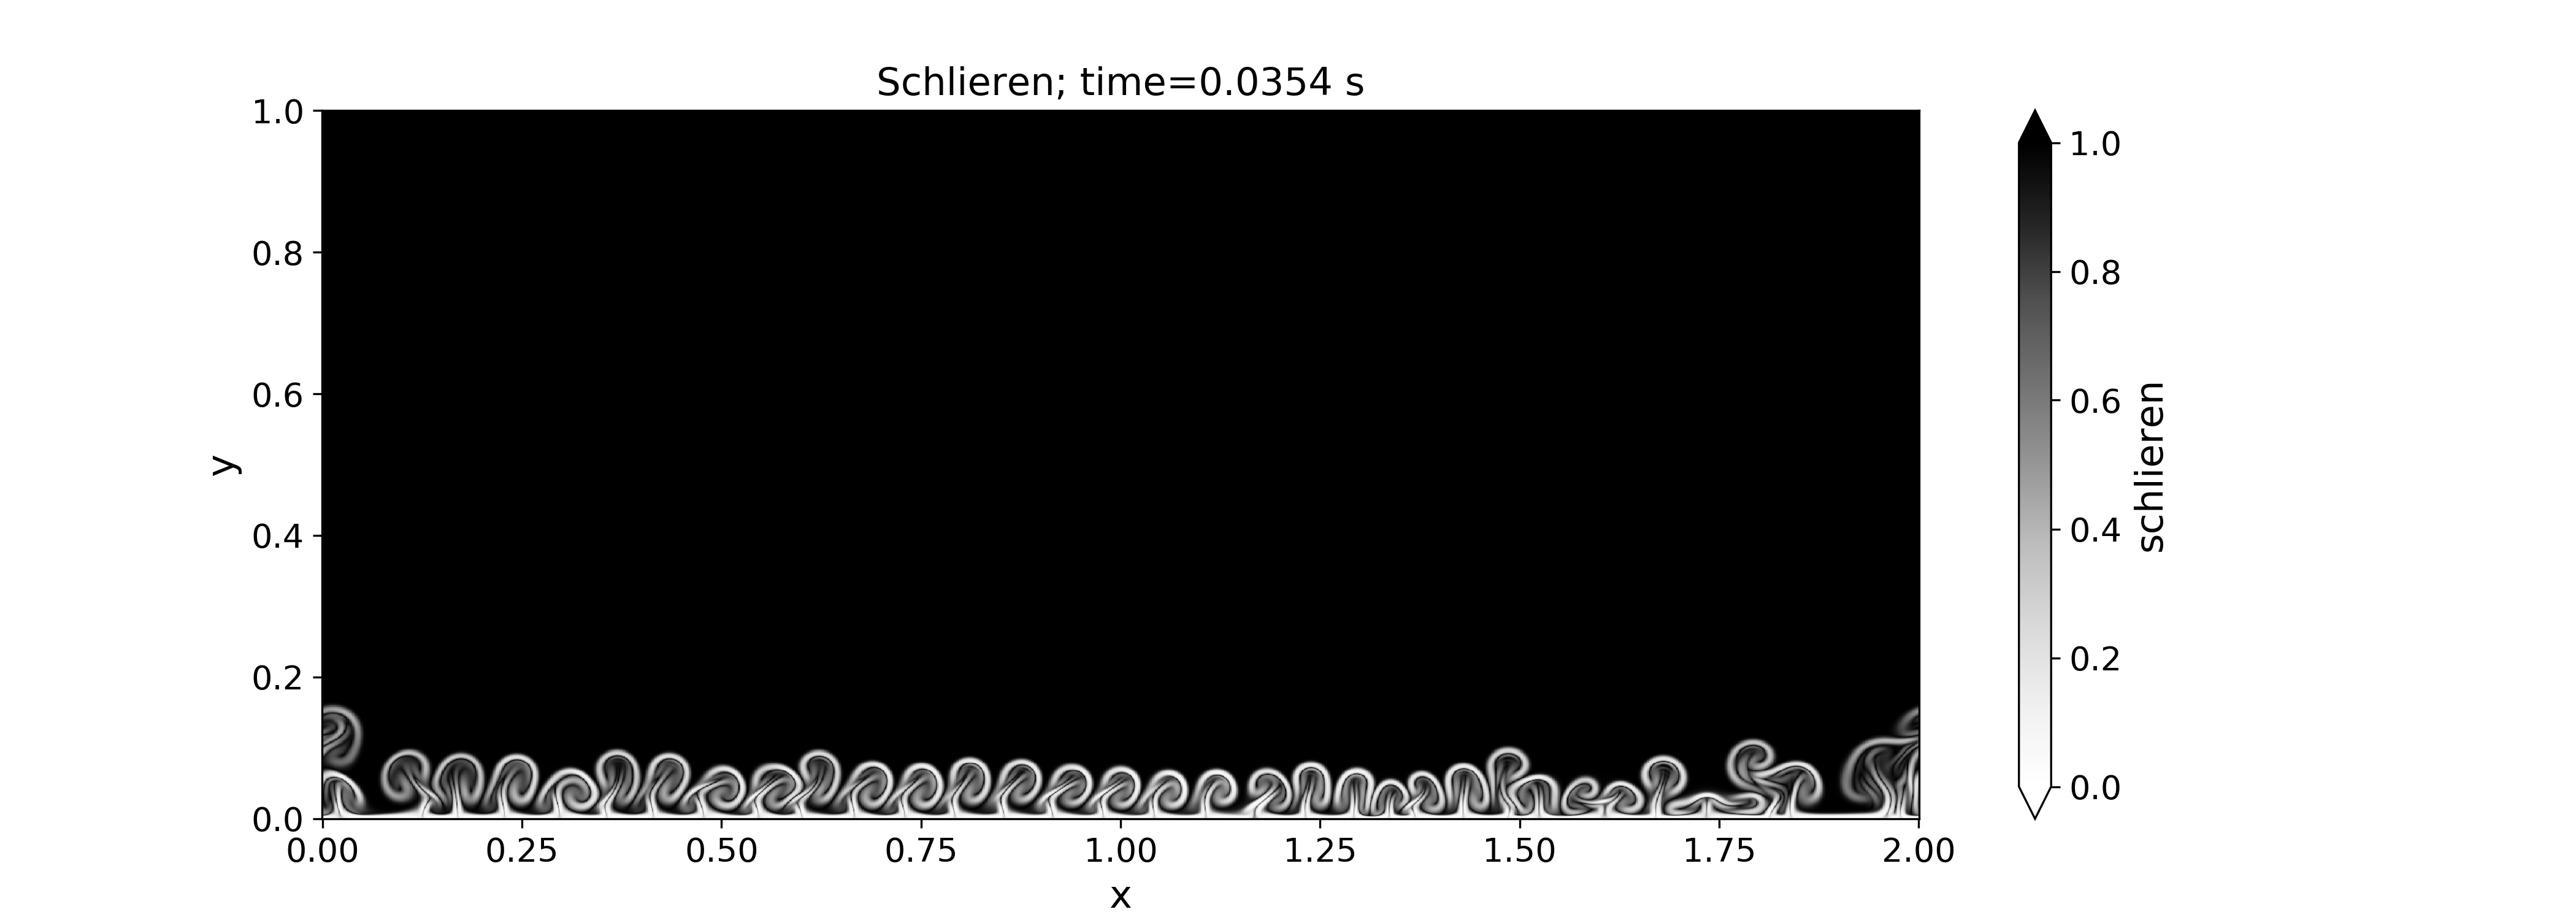
\includegraphics[scale=0.5]{sch_k50_frame_037}
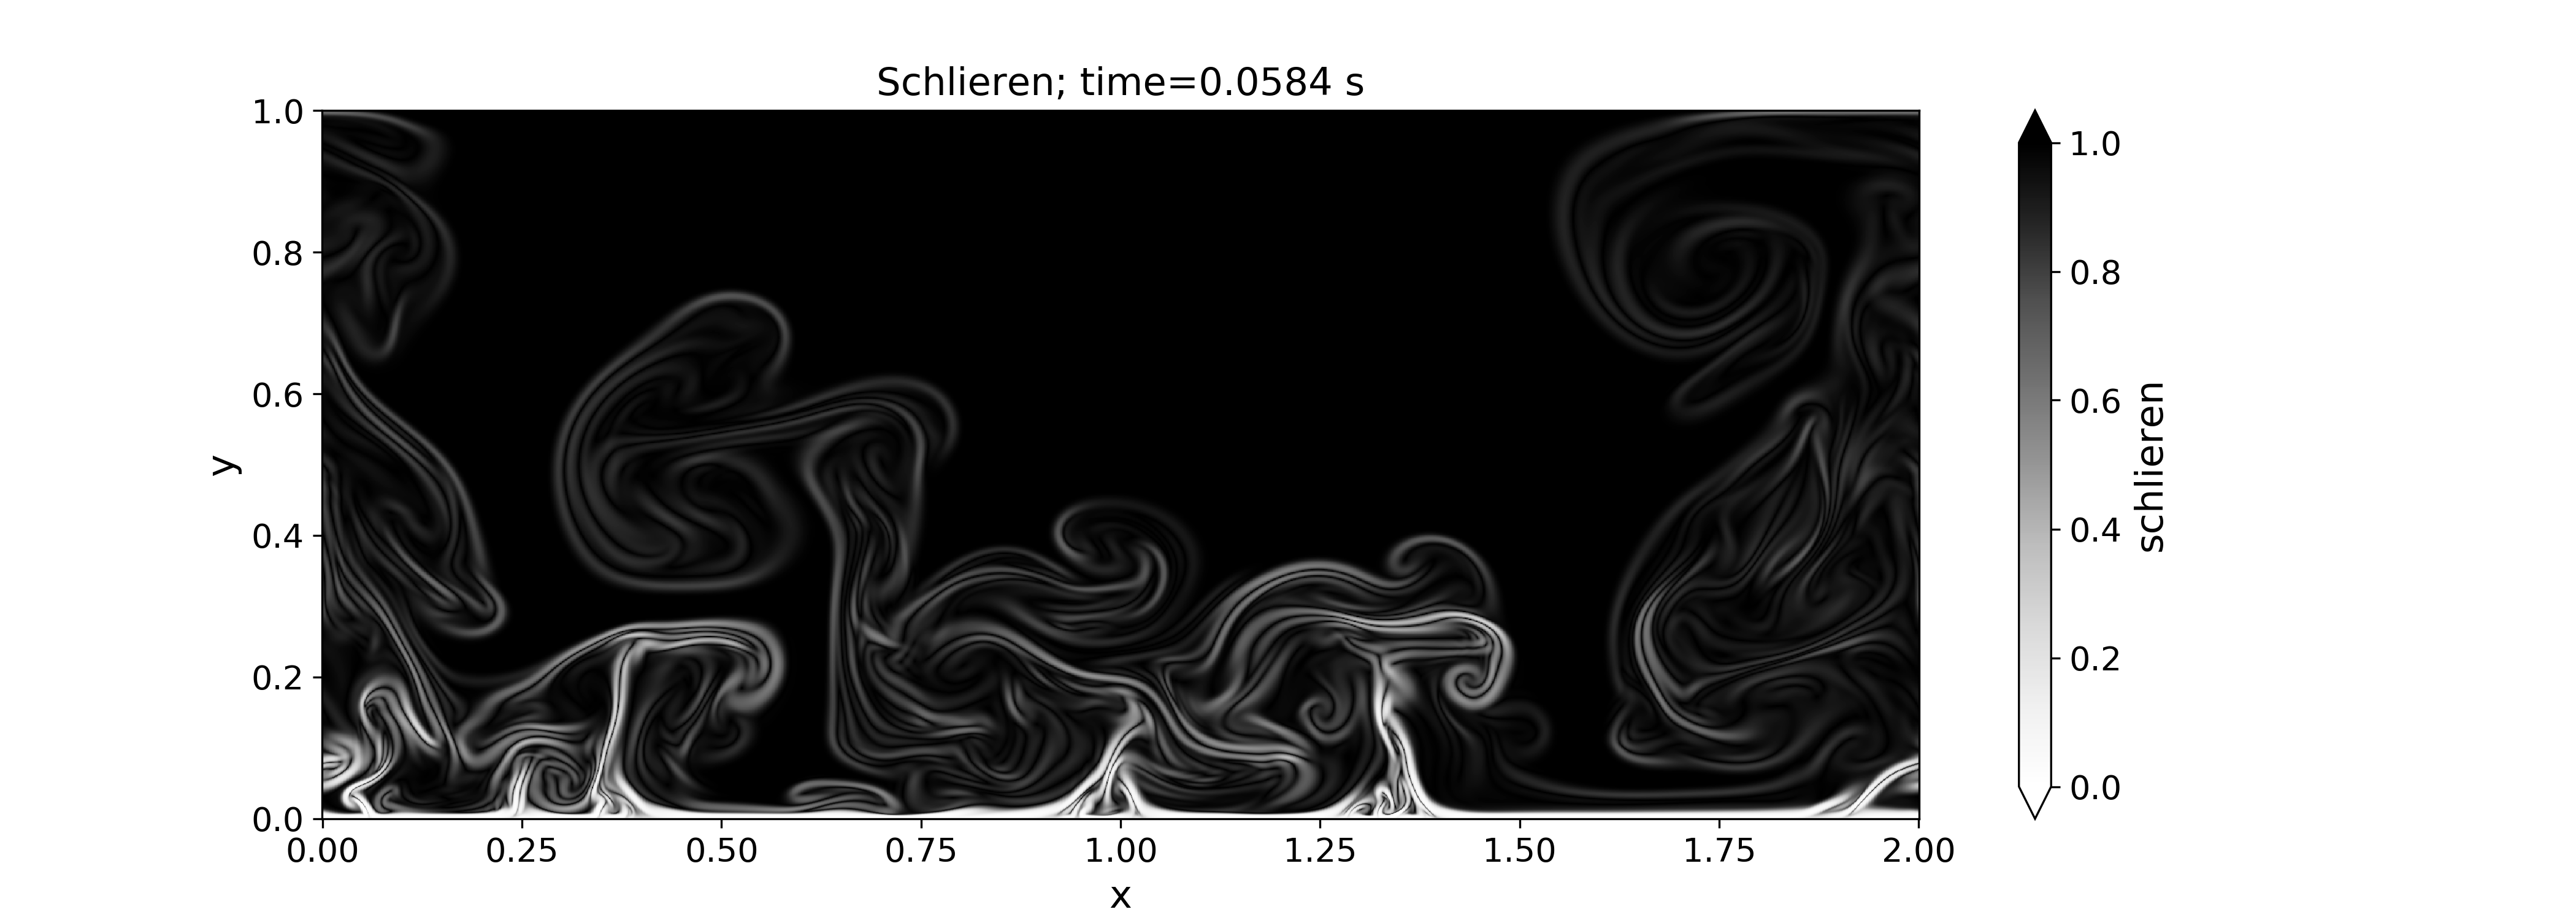
\includegraphics[scale=0.5]{sch_k50_frame_060}
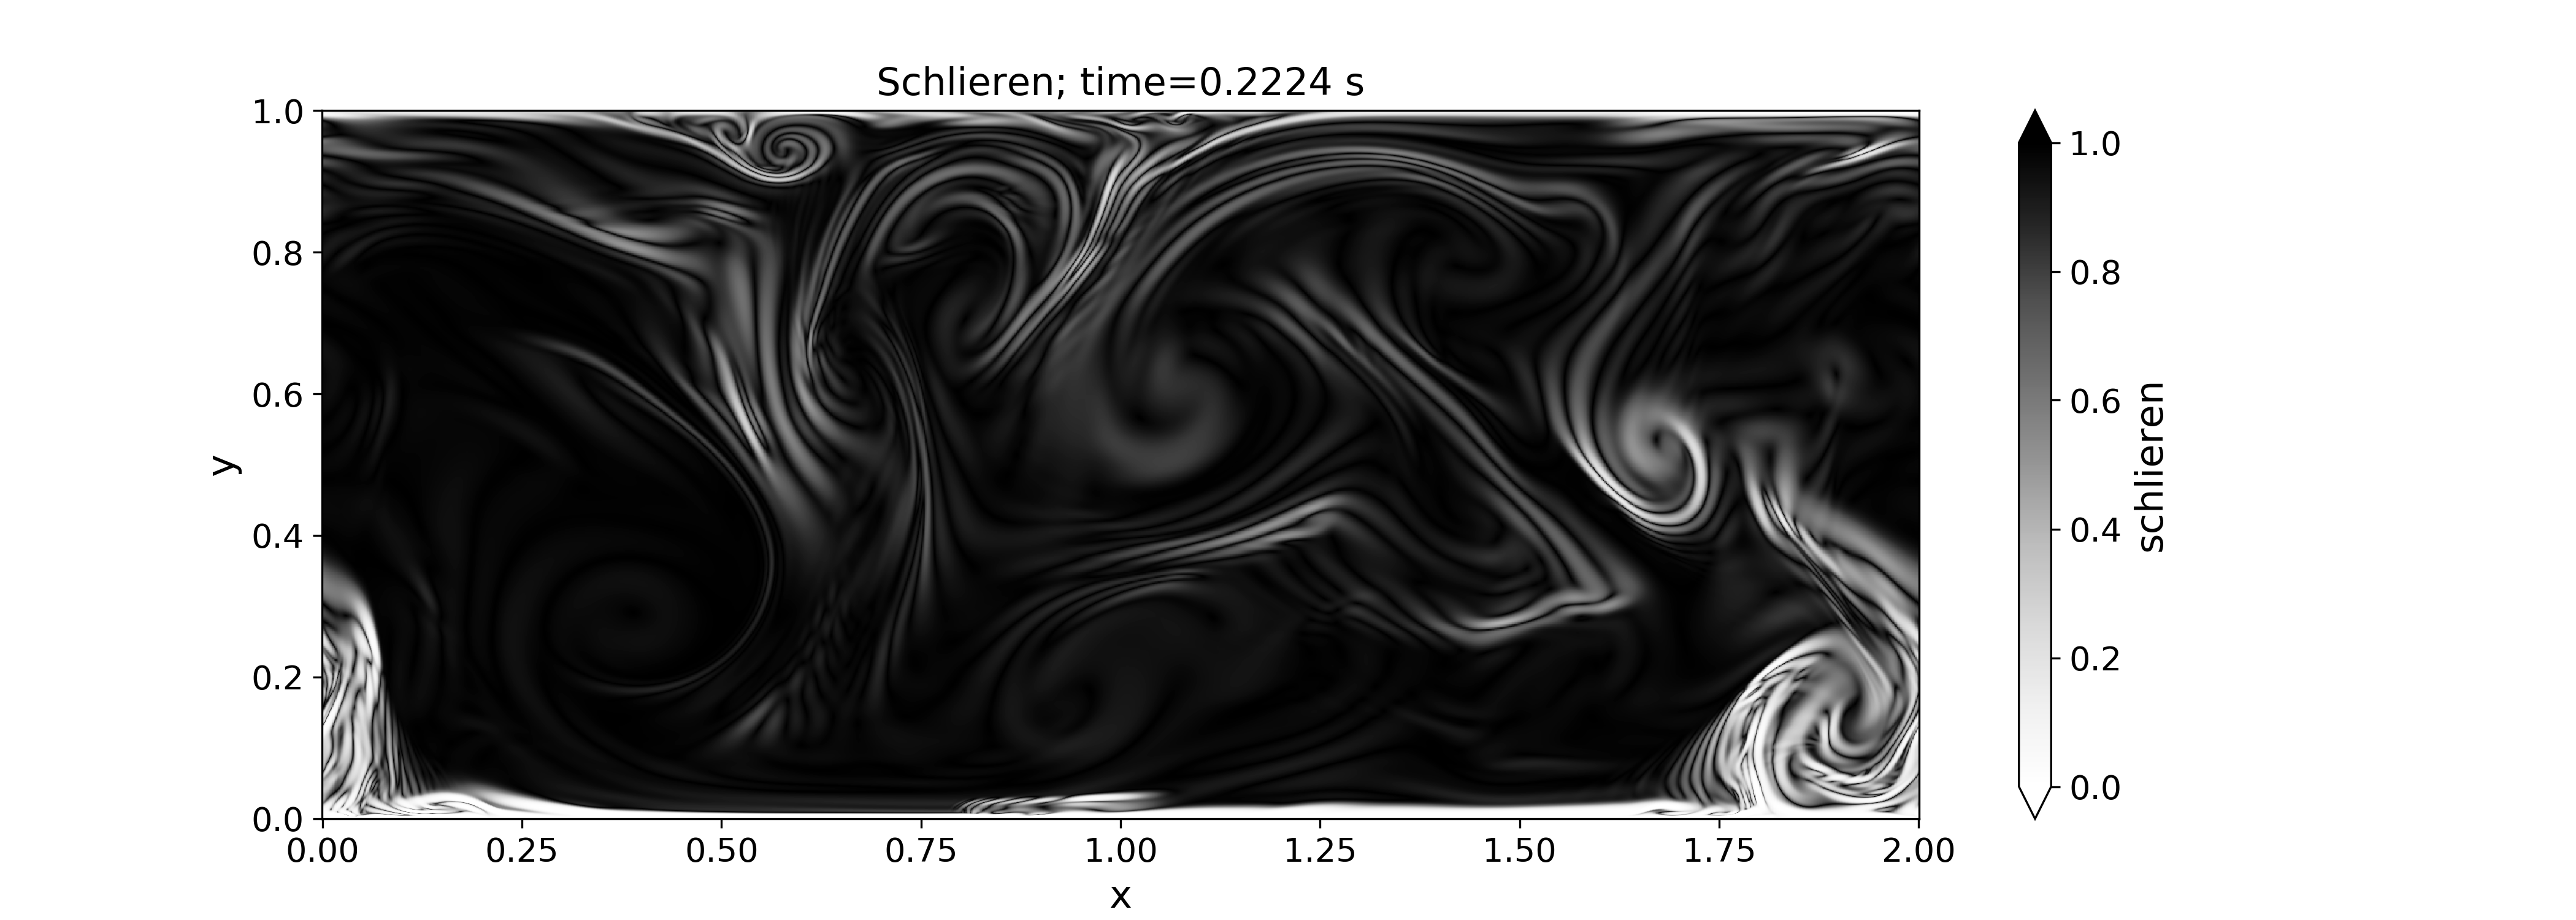
\includegraphics[scale=0.5]{sch_k50_frame_224}
\centering
\caption{Schlieren visualization with k=50}
\end{figure}

\begin{figure}[H]
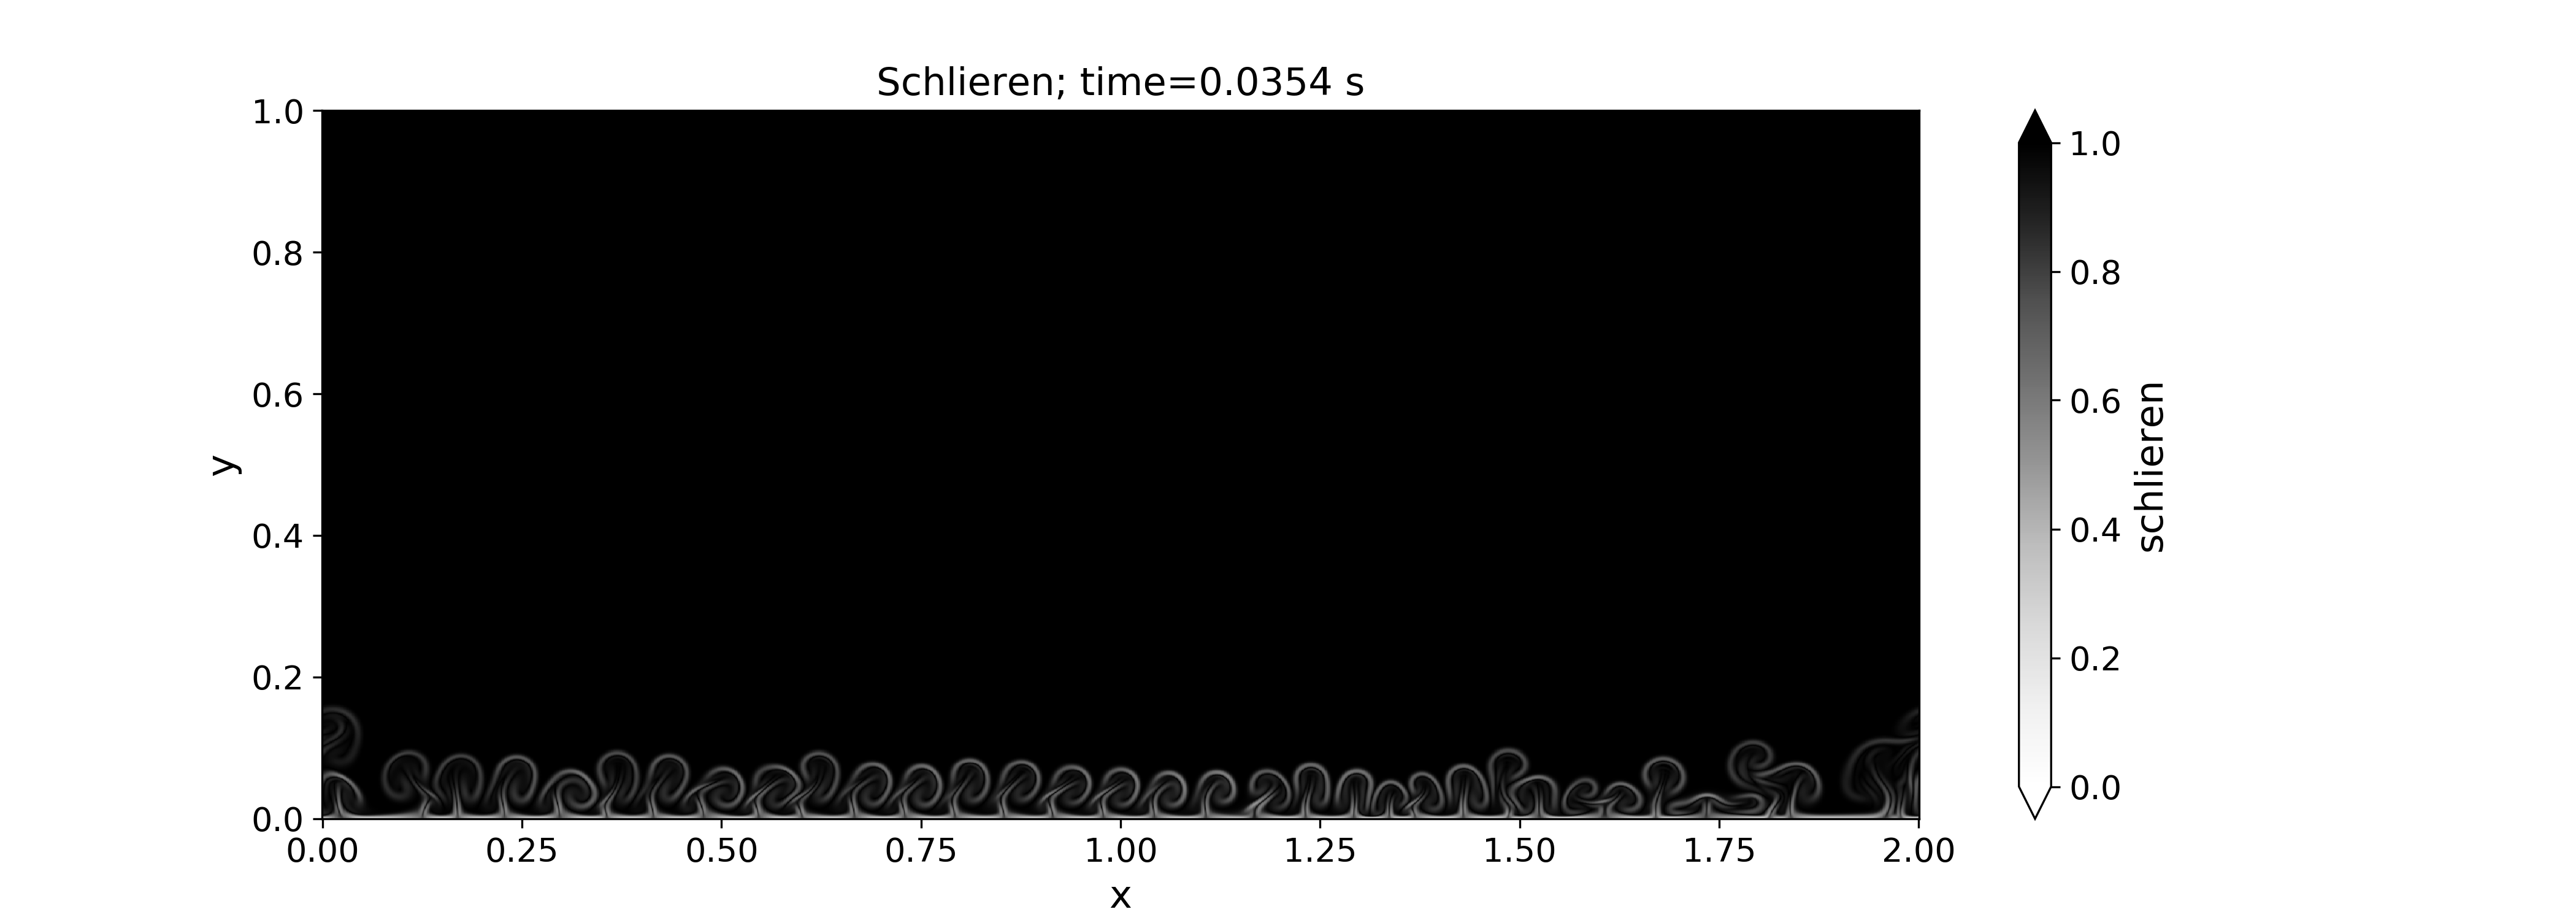
\includegraphics[scale=0.5]{sch_k10_frame_037}
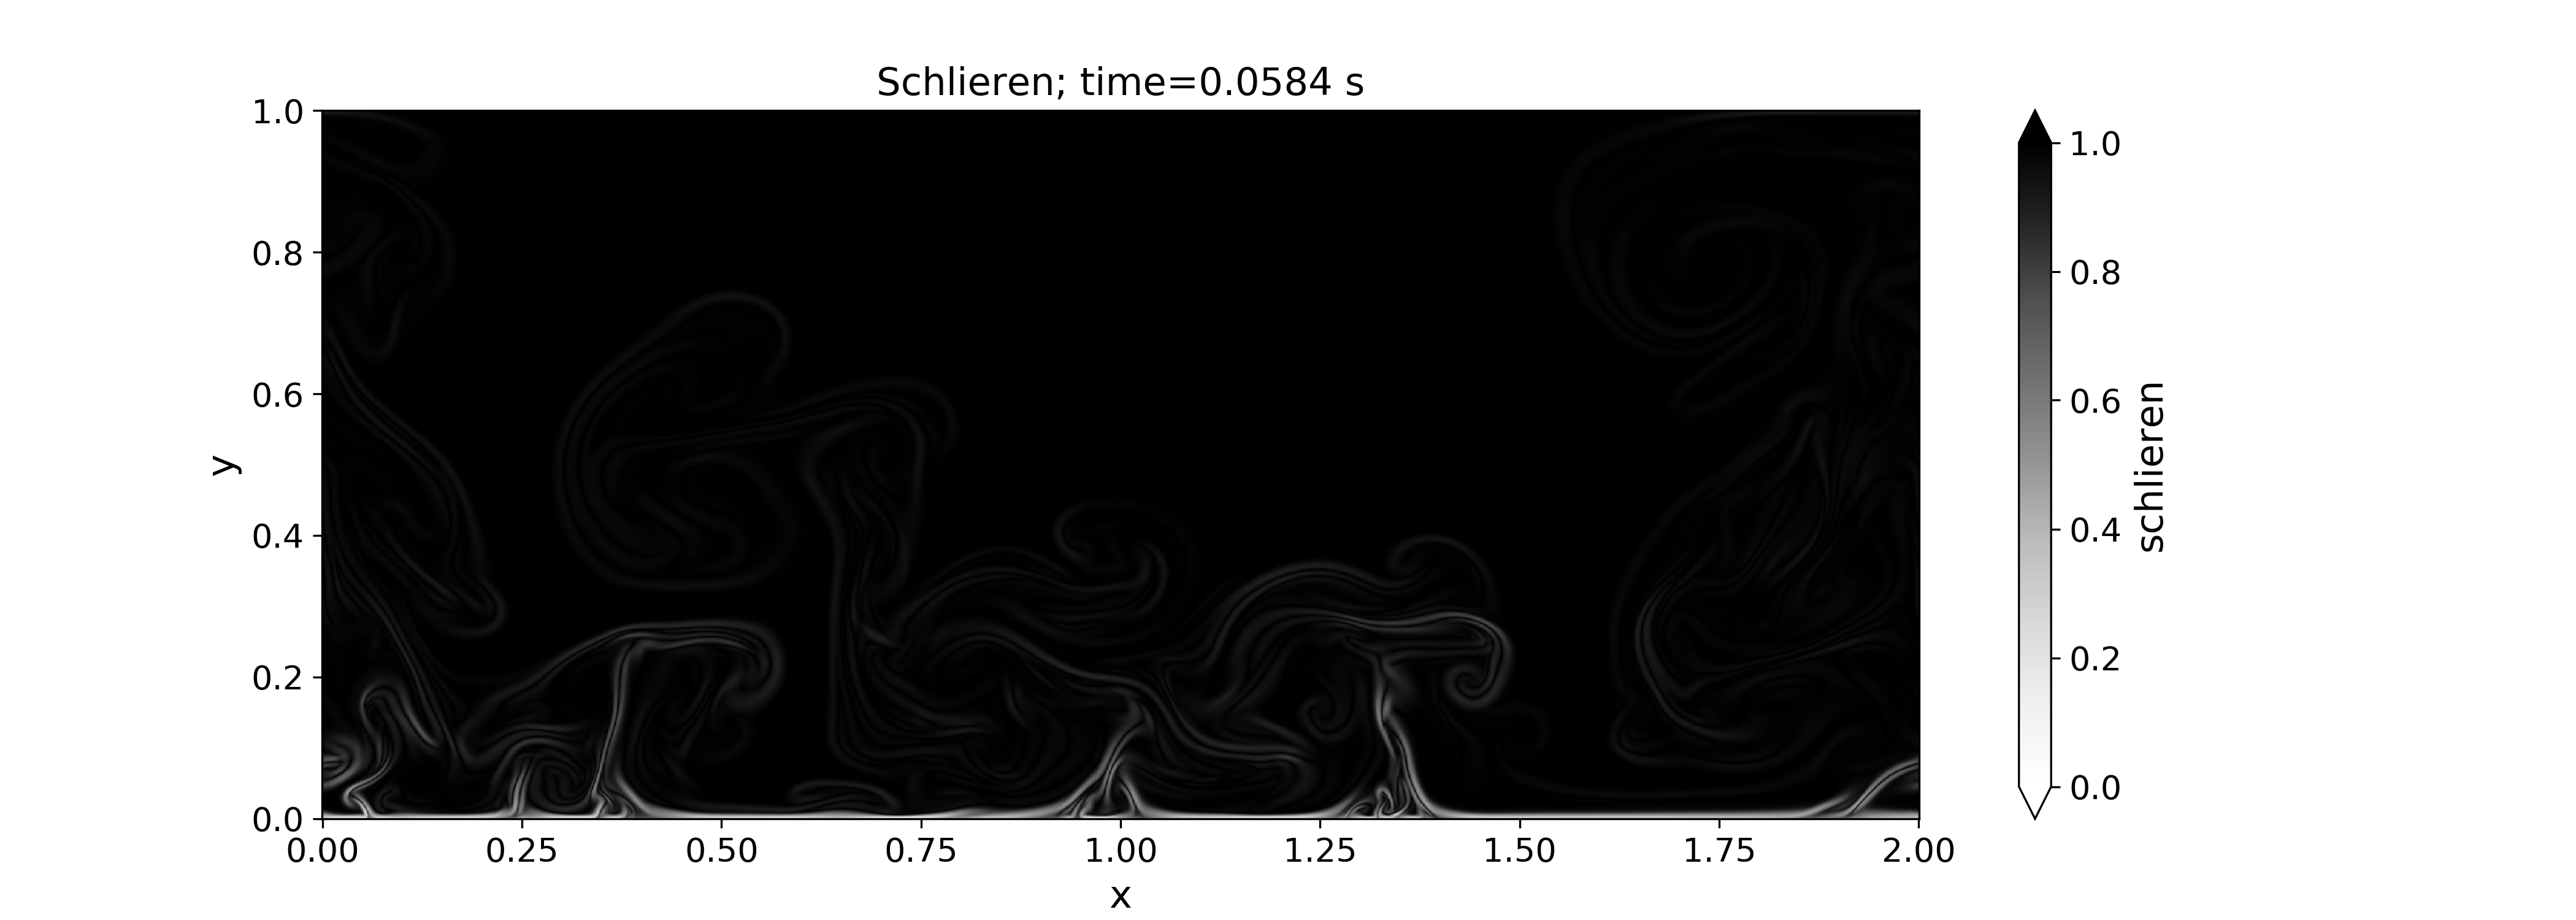
\includegraphics[scale=0.5]{sch_k10_frame_060}
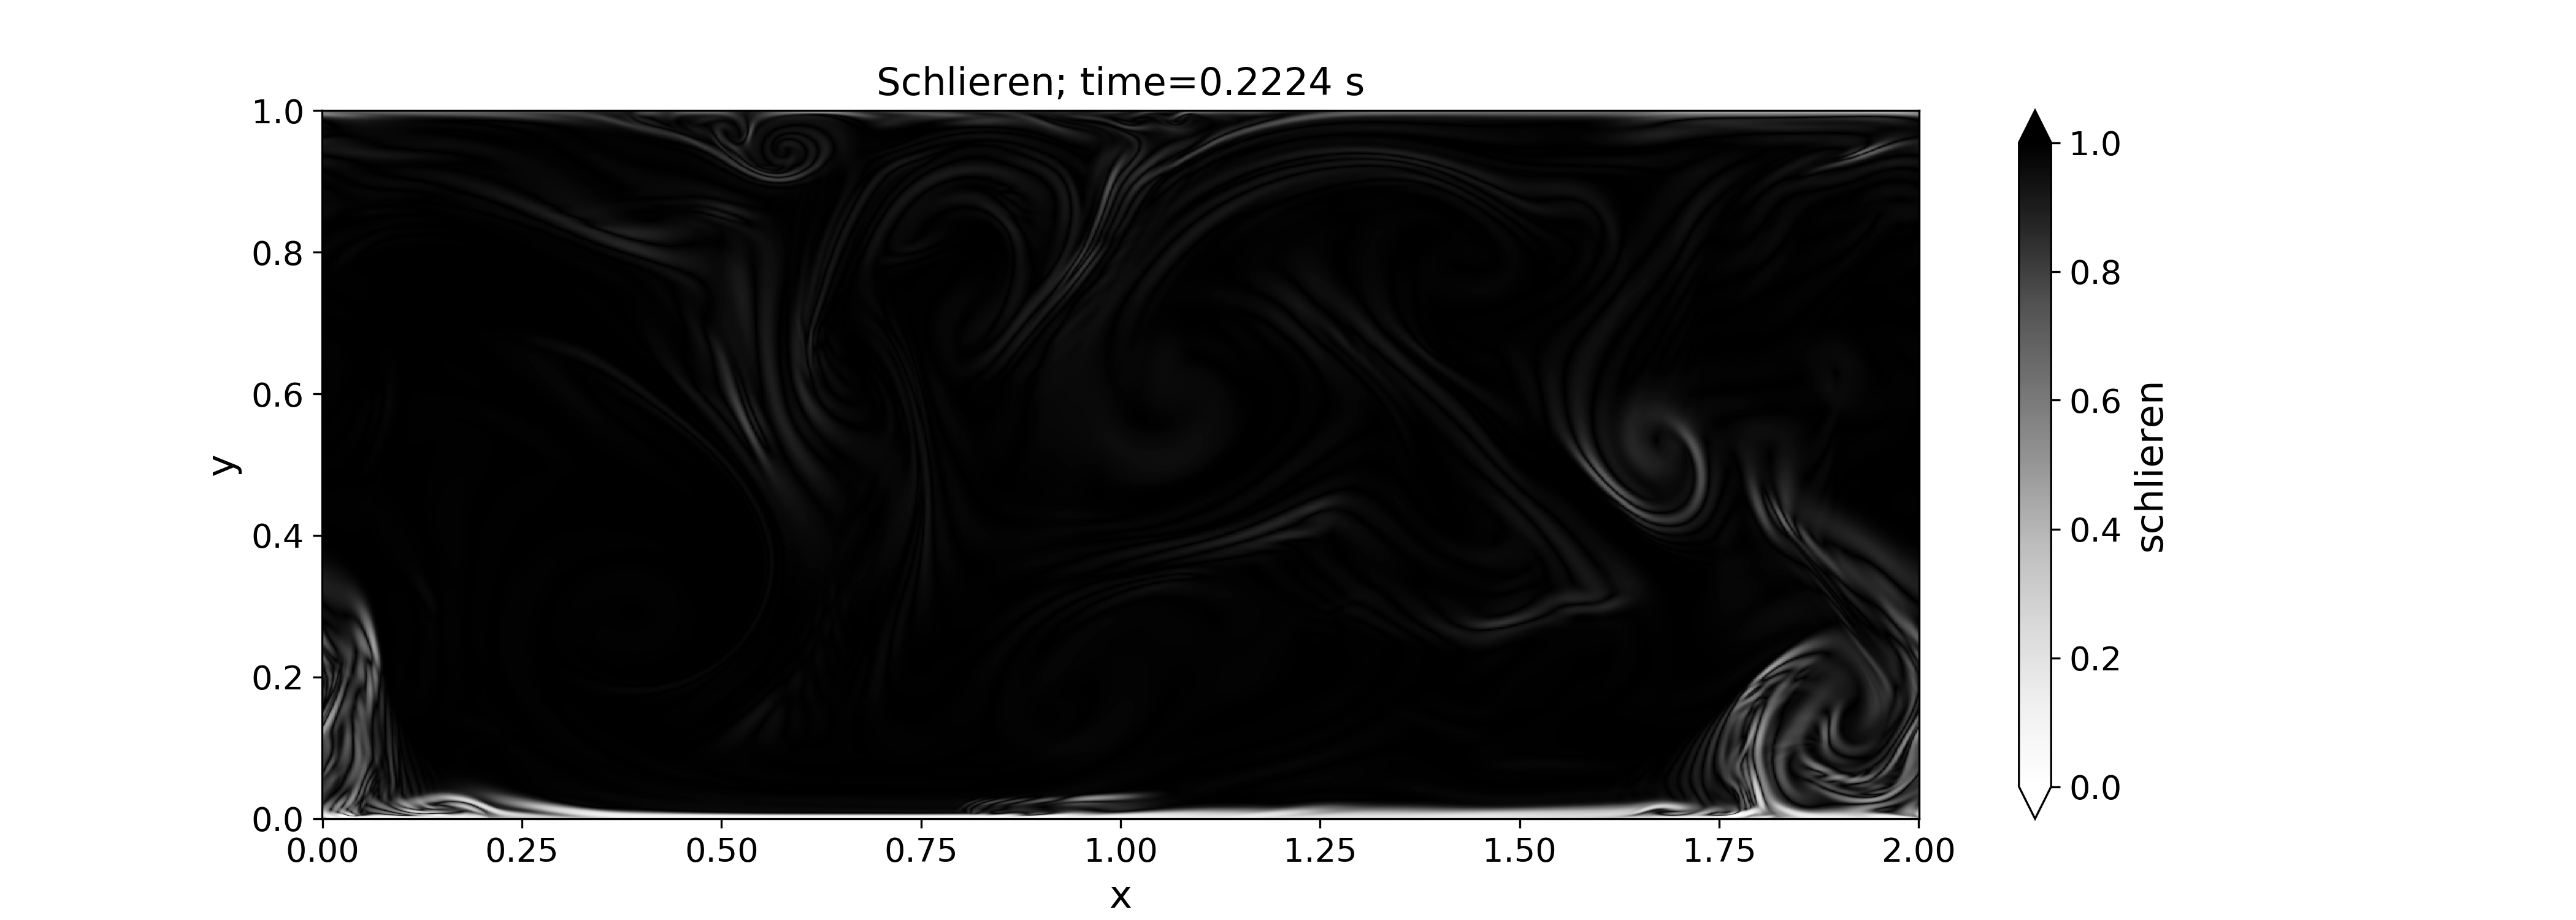
\includegraphics[scale=0.5]{sch_k10_frame_224}
\centering
\caption{Schlieren visualization with k=10}
\end{figure}

\subsection{Nusselt number}

Finally we compute the Nusselt number which indicates the ratio of convective heat transfer to conductive heat transfer. After $t > 0.005$ the Nusselt number settles around 130. Its magnitude is consistent with existing literature [2].

\begin{figure}[H]
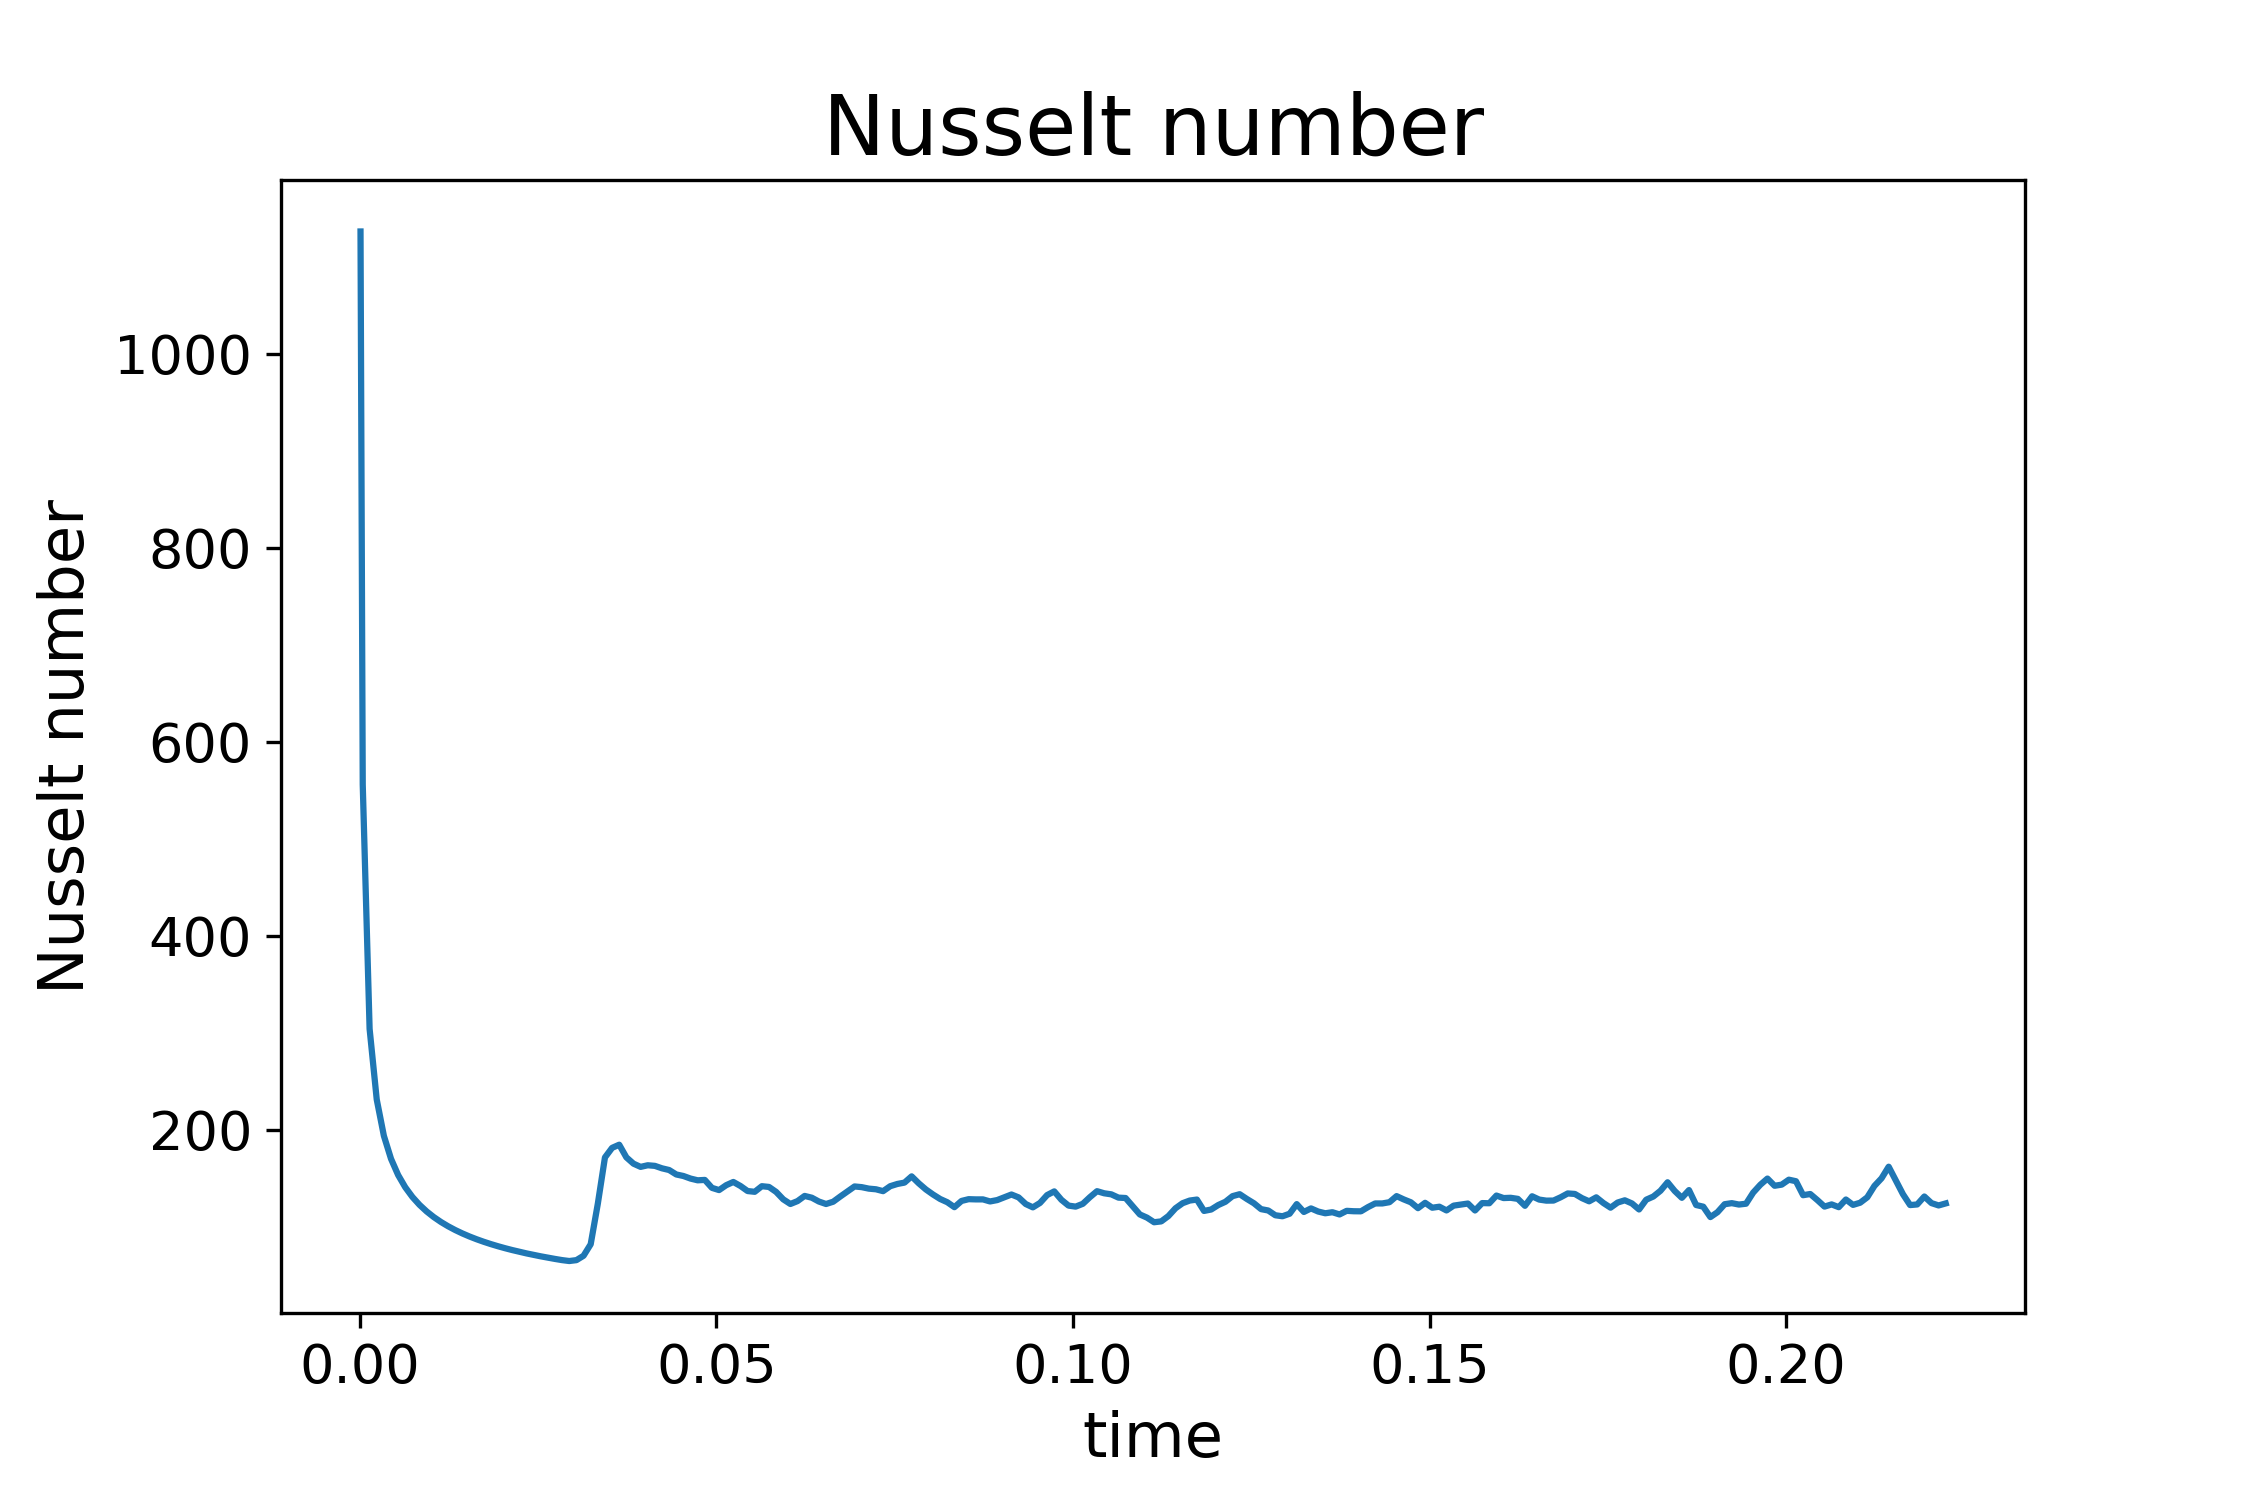
\includegraphics[scale=0.5]{Nusselt_number}
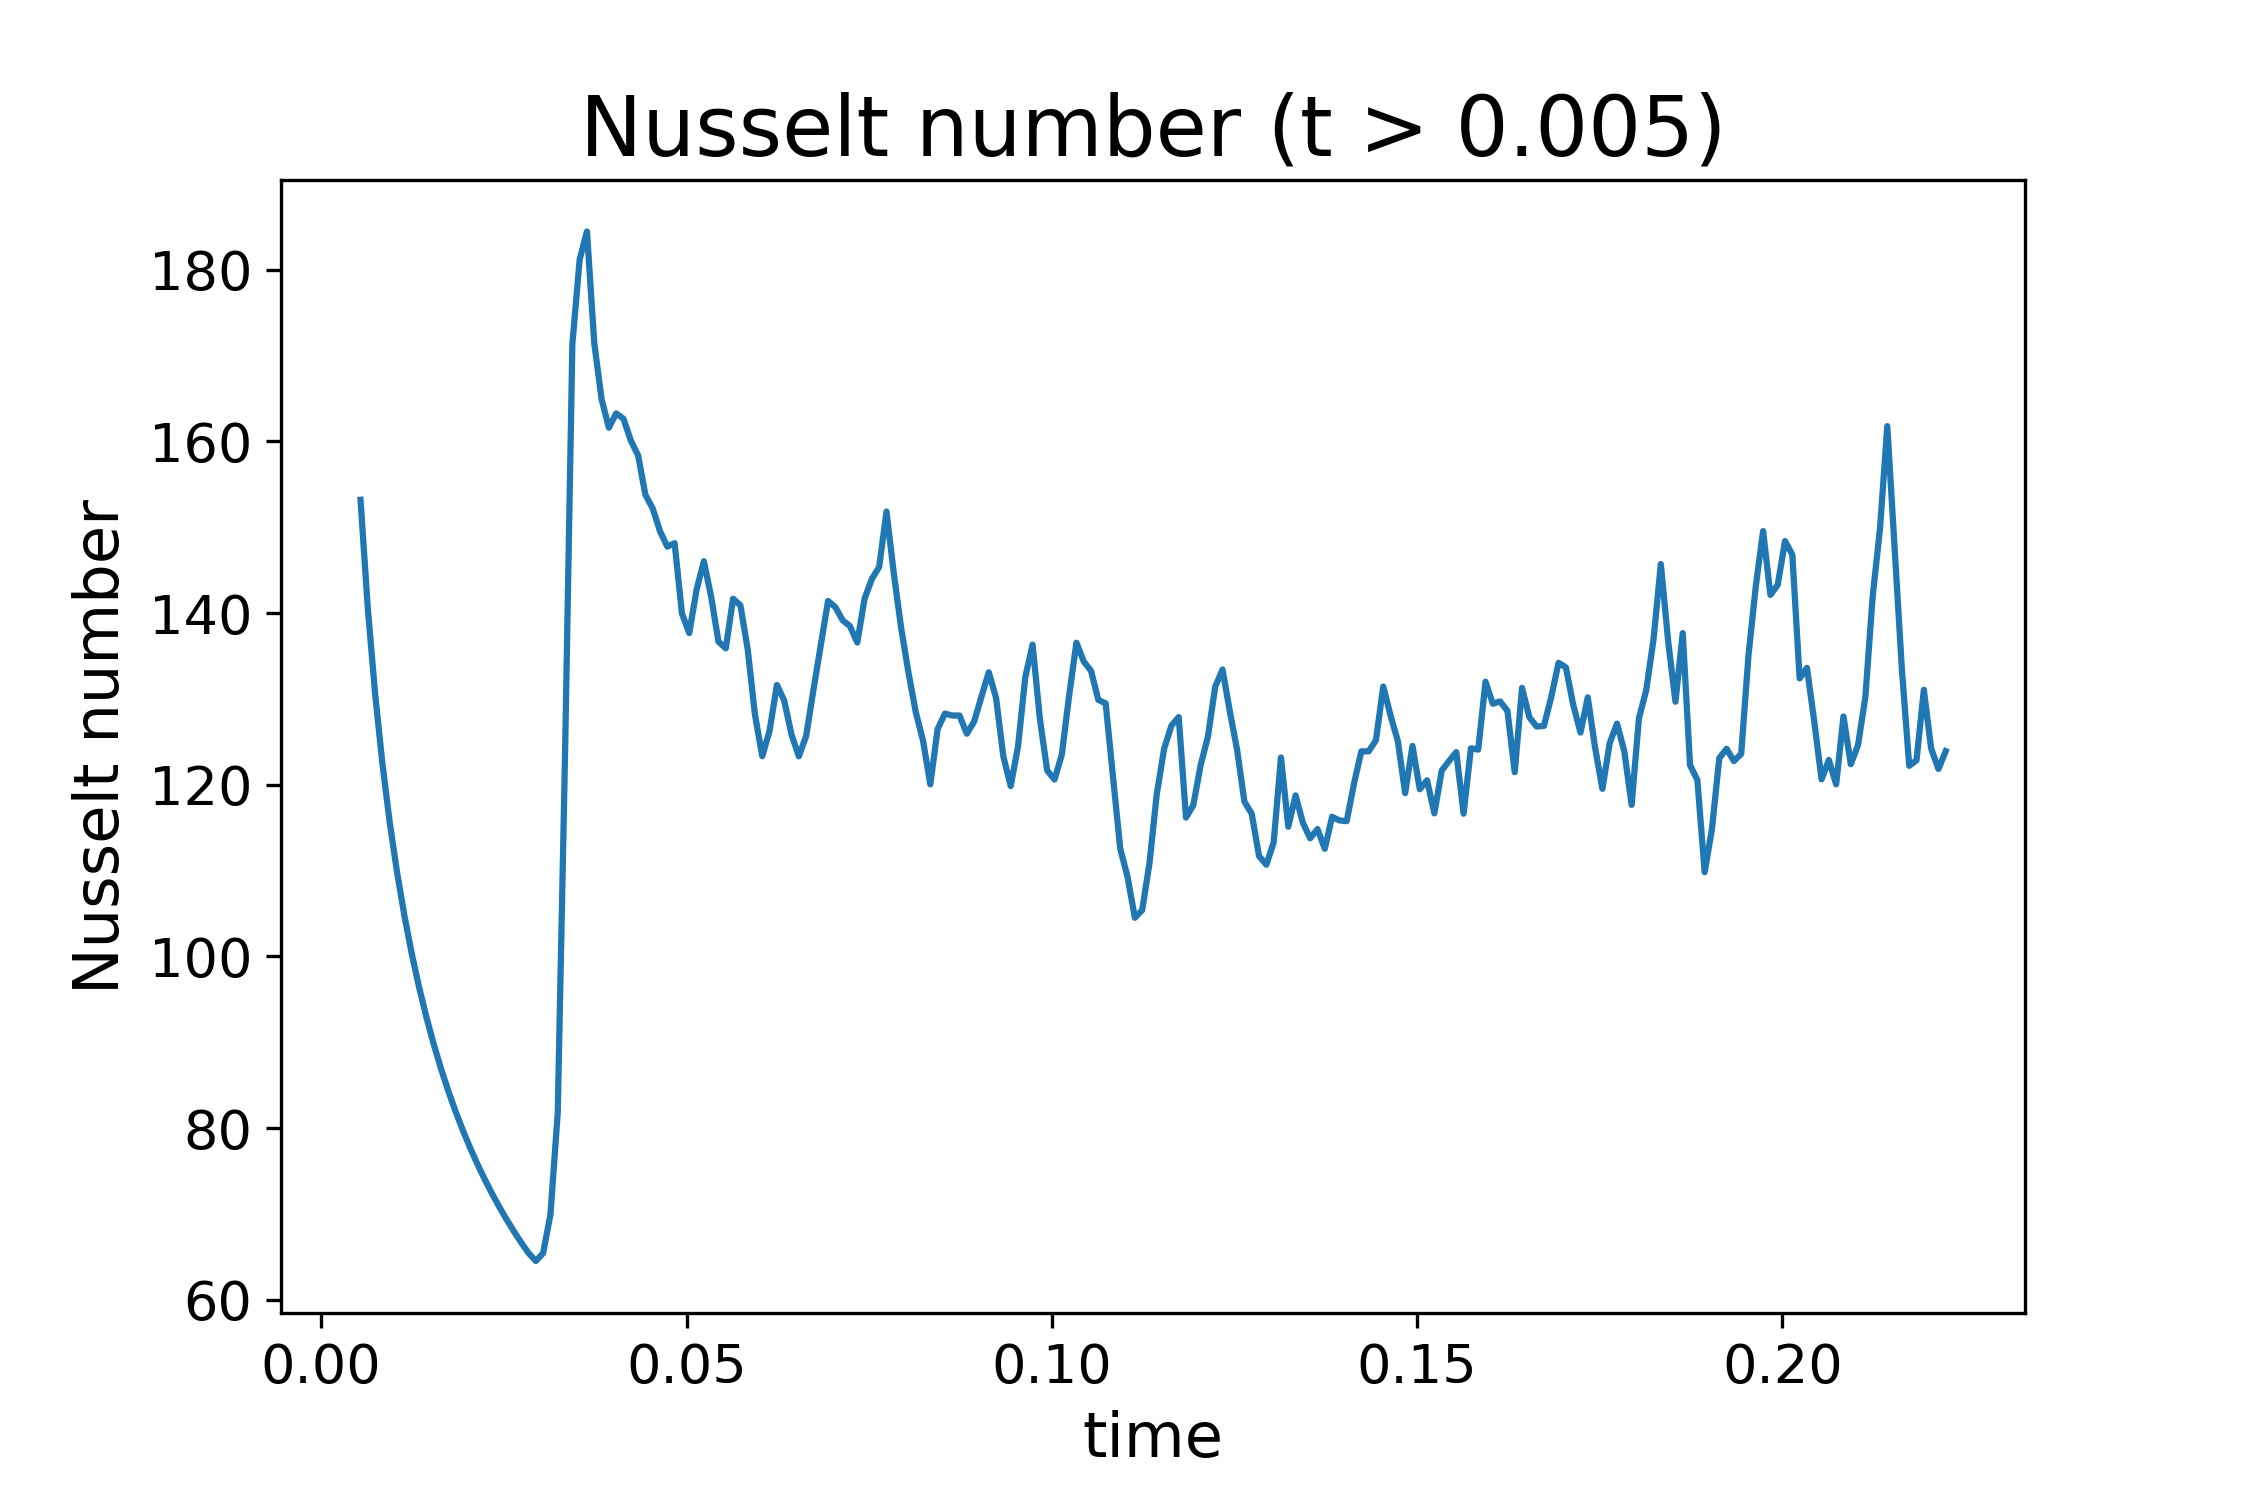
\includegraphics[scale=0.5]{Nusselt_number_truncate}
\centering
\caption{Nusselt number (time-dependent)}
\end{figure}
